\documentclass[12pt]{article}

\newif\ifdraft\drafttrue  % set true to show comments
% \newif\ifdraft\draftfalse  % set true to show comments
\newif\ifanon\anonfalse    % set true to suppress names, etc.
\newif\ifappendices\appendicesfalse

%\PassOptionsToPackage{usenames,dvipsnames,svgnames,table}{xcolor}

\usepackage[usenames,dvipsnames,svgnames,table]{xcolor}
\usepackage{amsmath}
\usepackage[capitalise]{cleveref}
\usepackage{makecell}%To keep spacing of text in tables
\usepackage{nccmath}
\usepackage{mathtools}
\usepackage{bussproofs}
\usepackage{varwidth}
\usepackage{amsthm}
\usepackage{csvsimple}
\usepackage{thmtools,thm-restate}
\usepackage{changepage}
\usepackage{booktabs}
\usepackage{amssymb}
\usepackage{enumitem}
\usepackage{multirow,bigdelim}
\usepackage{multicol}
\usepackage{siunitx}
\usepackage{listings}
\usepackage{letltxmacro}
\usepackage{sansmath}
\usepackage{url}
\usepackage{flushend}
\usepackage{microtype}
\usepackage[utf8]{inputenc}
\usepackage{mathpartir}
\usepackage{empheq}
\usepackage{array}
\usepackage{pgfplots}
\usepackage{stmaryrd}
\usepackage{courier}
\usepackage{qtree}
\usepackage[normalem]{ulem}
\usepackage{relsize}
\usepackage{tikz}
\usepackage{algorithm}
\usepackage[noend]{algpseudocode}
\usepackage{graphicx}
\usepackage{subcaption}
\usepackage{textcomp}
\usepackage{tabularx}
\usepackage{stackengine}
\usepackage{caption}
\usepackage{wrapfig}
\usepackage{remreset}
\usepackage{tabulary}
\usepackage{xspace}
\usepackage{bbm}
\usepackage{fullpage}
\usepackage[explicit]{titlesec}
\usepackage{longtable}

% \renewcommand*\thesection{\arabic{section}.0}
% \renewcommand*\thesubsection{\arabic{section}.\arabic{subsection}}

% Colors
\definecolor{dkblue}{rgb}{0,0.1,0.5}
\definecolor{dkgreen}{rgb}{0,0.6,0}
\definecolor{dkred}{rgb}{0.6,0,0}
\definecolor{dkpurple}{rgb}{0.2,0,0.4}
\definecolor{olive}{rgb}{0.4, 0.4, 0.0}
\definecolor{teal}{rgb}{0.0,0.5,0.5}
\definecolor{orange}{rgb}{0.9,0.6,0.2}
\definecolor{lightyellow}{RGB}{255, 255, 240}
\definecolor{vlightyellow}{RGB}{255, 255, 245}
\definecolor{lightgreen}{RGB}{235, 255, 240}
\definecolor{vlightgreen}{RGB}{247, 255, 250}
\definecolor{lightblue}{RGB}{245, 255, 255}
\definecolor{vlightblue}{RGB}{250, 255, 255}
\definecolor{teal}{RGB}{141,211,199}
\definecolor{darkbrown}{RGB}{121,37,0}

\newtheorem*{theorem*}{Theorem}
\newenvironment{centermath}
 {\begin{center}$\displaystyle}
 {$\end{center}}
\setcellgapes{4pt}%parameter for the spacing

\lstset{ language=Caml, basicstyle=\upshape\sffamily,
keywordstyle=\upshape\sffamily\color{dkpurple}, keepspaces=true,
framexleftmargin=1ex, framexrightmargin=1ex, showstringspaces=true,
commentstyle=\itshape\rmfamily,
emph={rep,iterate,synth,collapse,perm,squash,normalize,using,ins,del,lens,let,get,put,rquot,lquot,id,swap,concat,or,disconnect,merge_left,merge_right,const},
emphstyle=\upshape\sffamily\color{dkpurple}, 
columns=fullflexible,
mathescape, 
xleftmargin=1.5em,
% BCP: I find this distracting:
stringstyle=\sffamily\color{dkblue},
}
\makeatletter
     \let\lst@oldvisiblespace\lst@visiblespace
     \def\lst@visiblespace{\,\lst@oldvisiblespace\,}
\makeatother

\setlength{\belowdisplayskip}{0pt} \setlength{\belowdisplayshortskip}{0pt}
\setlength{\abovedisplayskip}{0pt} \setlength{\abovedisplayshortskip}{0pt}

\usetikzlibrary{
  er,
  matrix,
  shapes,
  arrows,
  positioning,
  fit,
  calc,
  pgfplots.groupplots,
  arrows.meta
}
\tikzset{>={Latex}}

%%%% Hyperlinks – must come late!
%\usepackage[pdftex,%
%            pdfpagelabels,%
%            linkcolor=blue,%
%            citecolor=blue,%
%            filecolor=blue,%
%            urlcolor=blue]
%           {hyperref}

% Colors
\definecolor{dkblue}{rgb}{0,0.1,0.5}
\definecolor{dkgreen}{rgb}{0,0.6,0}
\definecolor{dkred}{rgb}{0.6,0,0}
\definecolor{dkpurple}{rgb}{0.4,0,0.6}
\definecolor{olive}{rgb}{0.4, 0.4, 0.0}
\definecolor{teal}{rgb}{0.0,0.5,0.5}
\definecolor{orange}{rgb}{0.9,0.6,0.2}
\definecolor{lightyellow}{RGB}{255, 255, 179}
\definecolor{lightgreen}{RGB}{170, 255, 220}
\definecolor{teal}{RGB}{141,211,199}
\definecolor{darkbrown}{RGB}{121,37,0}

% remove whitespace before and after multicols
\setlength{\multicolsep}{0pt}

% renewtheorem https://tex.stackexchange.com/questions/103013/is-there-a-renewtheorem-equivalent-of-renewcommand-using-amsthm-and-not-ntheo
\makeatletter
\def\renewtheorem#1{%
  \expandafter\let\csname#1\endcsname\relax
  \expandafter\let\csname c@#1\endcsname\relax
  \gdef\renewtheorem@envname{#1}
  \renewtheorem@secpar
}
\def\renewtheorem@secpar{\@ifnextchar[{\renewtheorem@numberedlike}{\renewtheorem@nonumberedlike}}
\def\renewtheorem@numberedlike[#1]#2{\newtheorem{\renewtheorem@envname}[#1]{#2}}
\def\renewtheorem@nonumberedlike#1{  
\def\renewtheorem@caption{#1}
\edef\renewtheorem@nowithin{\noexpand\newtheorem{\renewtheorem@envname}{\renewtheorem@caption}}
\renewtheorem@thirdpar
}
\def\renewtheorem@thirdpar{\@ifnextchar[{\renewtheorem@within}{\renewtheorem@nowithin}}
\def\renewtheorem@within[#1]{\renewtheorem@nowithin[#1]}
\makeatother

\pgfplotsset{
% override style for non-boxed plots
    % which is the case for both sub-plots
    every non boxed x axis/.style={} 
}

\newenvironment{mathprooftree}
  {\varwidth{.9\textwidth}\centering\leavevmode}
  {\DisplayProof\endvarwidth}

\newcommand{\FINISH}[3]{\ifdraft\textcolor{#1}{[#2: #3]}\fi}
\newcommand{\bcp}[1]{\FINISH{dkred}{B}{#1}}
\newcommand{\BCP}[1]{\FINISH{dkred}{B}{\bf #1}}
\newcommand{\afm}[1]{\FINISH{dkgreen}{A}{#1}}
\newcommand{\dpw}[1]{\FINISH{dkblue}{D}{#1}}
\newcommand{\saz}[1]{\FINISH{orange}{S}{#1}}
\newcommand{\ksf}[1]{\FINISH{teal}{K}{#1}}
\newcommand{\revised}[1]{\FINISH{dkred}{#1}}

\newcommand{\IE}{\emph{i.e.}}
\newcommand{\EG}{\emph{e.g.}}
\newcommand{\ETC}{\emph{etc.}}

\theoremstyle{definition}
\renewtheorem{theorem}{Theorem}
\newtheorem{mylemma}{Lemma}
\renewtheorem{corollary}{Corollary}
\renewtheorem{conjecture}{Conjecture}
\renewtheorem{definition}{Definition}
\newtheorem{property}{Property}
\theoremstyle{plain}
\theoremstyle{remark}
\newtheorem{subcase}{Subcase}
\theoremstyle{remark}
\newtheorem{case}{Case}
\makeatletter
\@addtoreset{subcase}{case}
\@addtoreset{case}{mylemma}
\@addtoreset{case}{theorem}
\@addtoreset{case}{corollary}
\@addtoreset{case}{definition}
\@addtoreset{case}{definition}
\@removefromreset{theorem}{section}
\makeatother

\algnewcommand\algorithmicswitch{\textbf{switch}}
\algnewcommand\algorithmicmatch{\textbf{match}}
\algnewcommand\algorithmiccase{\textbf{case}}
\algnewcommand\algorithmicwith{\textbf{with}}
\algnewcommand\algorithmicforeach{\textbf{foreach}}
\algnewcommand\Assert[1]{\State \algorithmicassert(#1)}%
% New "environments"
\algdef{SE}[SWITCH]{Switch}{EndSwitch}[1]{\algorithmicmatch\ #1\ \algorithmicwith}{\algorithmicend\ \algorithmicswitch}%
\algdef{SE}[CASE]{Case}{EndCase}[1]{$|~$ #1 $\rightarrow$}{\algorithmicend\ \algorithmiccase}%
\algdef{SE}[FOREACH]{ForEach}{EndForEach}[2]{\algorithmicforeach\ #1 $\in$ #2}{\algorithmicend\ \algorithmicforeach}%
\algdef{SE}[CaseTwo]{CaseTwo}{EndCaseTwo}[2]{$|~$ #1 $\rightarrow$ #2}{\algorithmicend\ \algorithmiccase}%
\algtext*{EndSwitch}%
\algtext*{EndCase}%
\algtext*{EndCaseTwo}%
\algtext*{EndSecondCase}%
\algtext*{EndForEach}%



\newcommand{\CF}[1]{\ensuremath{\mathsf{#1}}}         % Code Font
\newcommand{\SmallCF}[1]{{\small \mathsf{#1}}}
\newcommand{\PCF}[1]{\textproc{#1}}
\newcommand{\VarCF}[1]{{\color{darkbrown} \CF{#1}}}
\newcommand{\StringCF}[1]{\CF{\textcolor{blue}{#1}}}
\newcommand{\KW}[1]{\CF{\textcolor{dkpurple}{#1}}}
\newcommand{\Regex}{\ensuremath{\mathit{S}}\xspace}         % Regular Expression
\newcommand{\RegexType}{\ensuremath{\textit{Regex}}}
\newcommand{\EquivRegexType}{\ensuremath{\textit{Regex}/\sim}}
\newcommand{\BooleanAnd}{\ensuremath{~\wedge~}}
\newcommand{\BooleanOr}{\ensuremath{\vee}}
\newcommand{\BooleanImplies}{\ensuremath{\Rightarrow}}
\newcommand{\Rewrite}{\ensuremath{\rightarrow}}
\newcommand{\RewriteAtom}{\ensuremath{\Rewrite_\Atom}}
\newcommand{\RewriteDNF}{\ensuremath{\Rewrite_\DNFRegex}}
\newcommand{\ConcatDNF}{\ensuremath{\odot}}
\newcommand{\ConcatDNFOf}[2]{\ensuremath{#1\ConcatDNF#2}}
\newcommand{\BigConcatDNF}{\ensuremath{\bigodot}}
\newcommand{\ConcatSequence}{\ensuremath{\odot_{\Sequence}}}
\newcommand{\ConcatSequenceOf}[2]{\ensuremath{#1\ConcatSequence#2}}
\newcommand{\ConcatPermutation}{\ensuremath{\odot}}
\newcommand{\ConcatPermutationOf}[2]{\ensuremath{#1\ConcatPermutation#2}}
\newcommand{\SwapPermutation}{\ensuremath{\circledS}}
\newcommand{\SwapPermutationOf}[2]{\ensuremath{#1\SwapPermutation#2}}
\newcommand{\DistributePermutation}{\ensuremath{\otimes}}
\newcommand{\DistributePermutationOf}[2]{\ensuremath{#1\DistributePermutation#2}}
\newcommand{\DistributeSwapPermutation}{\ensuremath{\otimes^{\mathit{s}}}}
\newcommand{\DistributeSwapPermutationOf}[2]{\ensuremath{#1\DistributeSwapPermutation#2}}
\newcommand{\ConcatSequenceLens}{\ensuremath{\odot_{\SequenceLens}}}
\newcommand{\ConcatSequenceLensOf}[2]{\ensuremath{#1\ConcatSequenceLens#2}}
\newcommand{\ConcatDNFLens}{\ensuremath{\odot}}
\newcommand{\ConcatDNFLensOf}[2]{\ensuremath{#1\ConcatDNFLens#2}}
\newcommand{\SwapSequenceLens}{\ensuremath{\circledS_{\SequenceLens}}}
\newcommand{\SwapSequenceLensOf}[2]{\ensuremath{#1\SwapSequenceLens#2}}
\newcommand{\SwapDNFLens}{\ensuremath{\circledS}}
\newcommand{\SwapDNFLensOf}[2]{\ensuremath{#1\SwapDNFLens#2}}
\newcommand{\RepeatDNFOfTimes}[1]{\ensuremath{^{#1}}}
\newcommand{\RepeatDNFOf}[2]{\ensuremath{{#2}\RepeatDNFOfTimes{#1}}}
\newcommand{\RepeatDNFLensOfTimes}[1]{\ensuremath{^{#1}}}
\newcommand{\RepeatDNFLensOf}[2]{\ensuremath{{#2}\RepeatDNFLensOfTimes{#1}}}
\newcommand{\OrDNF}{\ensuremath{\oplus}}
\newcommand{\OrDNFOf}[3]{\ensuremath{#1\OrDNF_{#3}#2}}
\newcommand{\OrDNFLens}{\ensuremath{\oplus}}
\newcommand{\OrDNFLensOf}[2]{\ensuremath{#1\OrDNFLens#2}}
\newcommand{\PutRSym}{\ensuremath{\mathit{putr}}}
\newcommand{\PutLSym}{\ensuremath{\mathit{putl}}}
\newcommand{\PutRSymOf}[1]{\ensuremath{\PutRSym \App #1}}
\newcommand{\PutLSymOf}[1]{\ensuremath{\PutLSym \App #1}}
\newcommand{\RegexAlt}{\ensuremath{\mathit{T}}\xspace}         % Regular Expression
\newcommand{\RegexAltAlt}{\ensuremath{\mathit{U}}\xspace}         % Regular Expression
\newcommand{\Or}{\ensuremath{~|~}}
\newcommand{\RegexOr}[2]{\ensuremath{#1\Or#2}}
\newcommand{\SubN}{\textsubscript{n}}
\newcommand{\RegexConcat}[2]{\ensuremath{#1\cdot#2}}
\newcommand{\EmptyString}{\ensuremath{\epsilon}}
\newcommand{\StringConcat}[2]{\ensuremath{#1\cdot#2}}
\newcommand{\HasSemantics}{\ensuremath{\triangleright}}
\newcommand{\DerivesLens}{\ensuremath{\vdash}}
\newcommand{\DerivesDNFLens}{\ensuremath{\vdash_{\DNFLens}}}
\newcommand{\DerivesSequenceLens}{\ensuremath{\vdash_{\SequenceLens}}}
\newcommand{\DerivesAtomLens}{\ensuremath{\vdash_{\AtomLens}}}
\newcommand{\DerivesStringRegex}{\ensuremath{\vdash}}
\newcommand{\DerivesAtomRewrite}{\ensuremath{\vdash}}
\newcommand{\DerivesDNFRewrite}{\ensuremath{\vdash}}
\newcommand{\Concat}{\ensuremath{\cdot}}
\newcommand{\Union}{\ensuremath{\cup}}
\newcommand{\Intersect}{\ensuremath{\cap}}
\newcommand{\BigUnion}{\ensuremath{\bigcup}}
\newcommand{\BigIntersect}{\ensuremath{\bigcap}}
\newcommand{\denot}[1]{\ensuremath{[ \! [#1] \! ]}}
\newcommand{\SemanticsOf}[1]{\ensuremath{[ \! [#1] \! ]}}
\newcommand{\SetOf}[1]{\ensuremath{\{#1\}}}
\newcommand{\RegexVariable}{\ensuremath{\mathit{U}}}   % User Defined
\newcommand{\RegexVariableAlt}{\ensuremath{\mathit{V}}}
\newcommand{\LensVariable}{\ensuremath{\mathit{L}}}
\newcommand{\ExampledRegex}{\ensuremath{\mathit{er}}} % Exampled Regex
\newcommand{\UnambigItOf}[1]{\ensuremath{#1^{*!}}}
\newcommand{\UnambigConcat}{\ensuremath{\Concat^!}}
\newcommand{\SequenceUnambigConcatOf}[1]{\ensuremath{\UnambigConcat(#1)}}
\newcommand{\UnambigConcatOf}[2]{\ensuremath{#1 \UnambigConcat #2}}
\newcommand{\UnambigOrOf}[2]{\ensuremath{\LanguageOf{#1} \cap \LanguageOf{#2} = \emptyset}}
\newcommand{\Atom}{\ensuremath{\mathit{A}}}          % Atoms
\newcommand{\AtomAlt}{\ensuremath{\mathit{B}}}
\newcommand{\AtomType}{\ensuremath{\mathit{Atom}}}
\newcommand{\App}{\ensuremath{\,}}
\newcommand{\Sequence}{\ensuremath{\mathit{SQ}}}
\newcommand{\SequenceType}{\ensuremath{\mathit{Sequence}}}
\newcommand{\LetIn}[2]{\ensuremath{\text{let } #1 = #2\text{ in }}}
\newcommand{\LetWhereIn}[3]{\ensuremath{\text{let } #1 = #2 \text{ where } #3 \text{ in }}}
\newcommand{\Where}{\ensuremath{\text{ where }}}
\newcommand{\ClauseAlt}{\ensuremath{\mathit{bl}}}       % Clauses
\newcommand{\SequenceAlt}{\ensuremath{\mathit{TQ}}}
\newcommand{\DNFRegex}{\ensuremath{\mathit{DS}}}         % Regular Expression
\newcommand{\DNFRegexAlt}{\ensuremath{\mathit{DT}}}    %Alt Regex
\newcommand{\DNFRegexType}{\ensuremath{\mathit{DNF}}}
\newcommand{\LensContext}{\ensuremath{\Gamma}}
\newcommand{\RegexContext}{\ensuremath{\Delta}}  % Context
\newcommand{\FullContext}{\ensuremath{\Delta, \Gamma}}
\newcommand{\String}{\ensuremath{\mathit{s}}\xspace}        % String
\newcommand{\StringAlt}{\ensuremath{\mathit{t}}}        % StringAlt
\newcommand{\StringAltAlt}{\ensuremath{\mathit{u}}}        % StringAltAlt
\newcommand{\ExampleNumberList}{\ensuremath{\mathit{enl}}} %Example Number List
\newcommand{\ExampleNumberListList}{\ensuremath{\mathit{enll}}}
\newcommand{\ExampleStringList}{\ensuremath{\mathit{esl}}}
\newcommand{\StringList}{\ensuremath{\mathit{sl}}}
\newcommand{\Natural}{\ensuremath{\mathit{n}}}
\newcommand{\Interleaving}[1]{\ensuremath{\mathit{interleaving}(#1)}}
\newcommand{\Interleave}{\ensuremath{\mathit{interleave}}}
\newcommand{\BinaryInterleave}[2]{\ensuremath{\mathit{interleave}(#1,#2)}}
\newcommand{\NAryInterleave}[2]{\ensuremath{\mathit{interleave}(#1,\ldots,#2)}}
\newcommand{\Combine}{\ensuremath{\mathit{combine}}}
\newcommand{\List}{\ensuremath{\mathit{l}}}
\newcommand{\ValidCombine}[2]{\ensuremath{\mathit{validcombine}(#1,#2)}}
\newcommand{\ValidRegexContext}[2]{\ensuremath{\mathit{validregexcontext}(#1,#2)}}
\newcommand{\Parent}[1]{\ensuremath{\mathit{parent}(#1)}}
\newcommand{\Parented}[1]{\ensuremath{mathit{parented}(#1)}}
\newcommand{\CombineString}[1]{\ensuremath{\mathit{combine}_{\ExampleStringList}(#1)}}
\newcommand{\CombineList}[1]{\ensuremath{\mathit{combine}_{\ExampleNumberListList}(#1)}}
\newcommand{\Length}[1]{\ensuremath{\mathit{len}(#1)}}
\newcommand{\Language}{\ensuremath{L}}
\newcommand{\LanguageOf}[1]{\ensuremath{\mathcal{L}(#1)}}
\newcommand{\LanguageUnderContextOf}[2]{\ensuremath{\Language{}_{#1}(#2)}}
\newcommand{\ParseTree}{\ensuremath{\mathit{p}}}
\newcommand{\ParseTreeAlt}{\ensuremath{\mathit{q}}}
\newcommand{\ParseTrees}{\ensuremath{\mathit{ps}}}
\newcommand{\ParseTreeAlts}{\ensuremath{\mathit{qs}}}
\newcommand{\StarParse}[1]{\ensuremath{\mathit{starparse}(#1)}}
\newcommand{\LeftChoiceParse}[1]{\ensuremath{\mathit{l}.(#1)}}
\newcommand{\RightChoiceParse}[1]{\ensuremath{\mathit{r}.(#1)}}
\newcommand{\RangeExcInc}[2]{\ensuremath{(#1,#2]}}
\newcommand{\RangeIncInc}[2]{\ensuremath{[#1,#2]}}

\newcommand{\Lens}{\ensuremath{\mathit{\ell}}\xspace}
\newcommand{\AtomLens}{\ensuremath{\mathit{al}}}
\newcommand{\IterateAtomType}{\textit{Iterate}}
\newcommand{\ConcatedAtomsLens}{\ensuremath{\mathit{cal}}}
\newcommand{\OredClausesLens}{\ensuremath{\mathit{ocl}}}
\newcommand{\ClauseLens}{\ensuremath{\mathit{cll}}}
\newcommand{\SequenceLens}{\ensuremath{\mathit{sql}}}
\newcommand{\SequenceLensType}{\ensuremath{\mathit{SequenceLens}}}
\newcommand{\DNFLens}{\ensuremath{\mathit{dl}}}
\newcommand{\DNFLensType}{\ensuremath{\mathit{DNFLens}}}
\newcommand{\AtomLensType}{\ensuremath{\mathit{AtomLens}}}
\newcommand{\SynSim}[2]{\ensuremath{#1 \sim_{\mathit{sym}} #2}}
\newcommand{\ExdSynSim}[3]{\ensuremath{#2 \sim_{\mathit{sym},#1} #3}}

\newcommand{\PermutationSetOf}[1]{\ensuremath{S_{#1}}}
\newcommand{\Permutation}{\ensuremath{\sigma}}

\newcommand{\Star}{\ensuremath{^*}}
\newcommand{\StarOf}[1]{\ensuremath{{#1}\Star}}
\newcommand{\ConstLens}{\ensuremath{\mathit{const}}}
\newcommand{\ConstLensOf}[2]{\ensuremath{\ConstLens(#1,#2)}}
\newcommand{\ConcatLens}{\ensuremath{\KW{concat}}}
\newcommand{\ConcatLensOf}[2]{\ensuremath{\ConcatLens(#1,#2)}}
\newcommand{\ConcatLensShortOf}[2]{\ensuremath{\mathit{c}(#1,#2)}}
\newcommand{\SwapLens}{\ensuremath{\KW{swap}}\xspace}
\newcommand{\SwapLensOf}[2]{\ensuremath{\SwapLens(#1,#2)}}
\newcommand{\SwapLensShortOf}[2]{\ensuremath{\mathit{s}(#1,#2)}}
\newcommand{\OrLens}{\ensuremath{\KW{or}}\xspace}
\newcommand{\OrLensOf}[2]{\ensuremath{\OrLens(#1,#2)}}
\newcommand{\IdentityLens}{\ensuremath{\KW{id}}}
\newcommand{\IdentityLensOf}[1]{\ensuremath{\IdentityLens(#1)}}
\newcommand{\IdentityLensShortT}{\ensuremath{\mathit{id}}}
\newcommand{\IdentityLensShortOf}[1]{\ensuremath{\IdentityLensShortT_{#1}}}
\newcommand{\IterateLens}{\ensuremath{\KW{iterate}}\xspace}
\newcommand{\IterateLensOf}[1]{\ensuremath{\mathit{\IterateLens(#1)}}}
\newcommand{\Identity}{\ensuremath{\mathit{id}}}
\newcommand{\Compose}{\ensuremath{\circ}}
\newcommand{\ComposeLensOf}[2]{\ensuremath{#1\mathrel{;}#2}}
\newcommand{\Disconnect}{\ensuremath{\KW{disc}}\xspace}
\newcommand{\DisconnectOf}[4]{\ensuremath{\Disconnect(#1,#2,#3,#4)}}
\newcommand{\MergeL}{\ensuremath{\KW{merge\_left}}\xspace}
\newcommand{\MergeLOf}[2]{\ensuremath{\MergeL(#1,#2)}}
\newcommand{\MergeR}{\ensuremath{\KW{merge\_right}}\xspace}
\newcommand{\MergeROf}[2]{\ensuremath{\MergeR(#1,#2)}}
\newcommand{\Invert}{\ensuremath{\KW{invert}}}
\newcommand{\InvertOf}[1]{\ensuremath{\Invert(#1)}}

% GRAMMAR OPERATORS
\newcommand{\GBar}{\ensuremath{~|~}}
\newcommand{\GIndent}{\hspace{.5in}}
\newcommand{\GEq}{\ensuremath{::=~}}
\newcommand{\GEmp}{\ensuremath{\cdot}}
\newcommand{\Perm}{\ensuremath{\mathit{Perm}}}
\newcommand{\Nats}{\ensuremath{\mathbb{N}}}

\newcommand{\InverseOf}[1]{\ensuremath{#1^{-1}}}
\newcommand{\FloorOf}[1]{\ensuremath{\lfloor#1\rfloor}}
\newcommand{\CeilOf}[1]{\ensuremath{\lceil#1\rceil}}
\newcommand{\OfType}{\ensuremath{:}}
\newcommand{\OfRewritelessType}{\ensuremath{\,\,\tilde{\OfType}\,\,}}
\newcommand{\MapsBetweenTypeOf}[2]{\ensuremath{#1 \Leftrightarrow #2}}
\newcommand{\ArrowTypeOf}[2]{\ensuremath{#1 \rightarrow #2}}
\newcommand{\SizeOf}[1]{\ensuremath{|#1|}}

\newcommand{\ToDNFRegex}{\ensuremath{\Downarrow}}
\newcommand{\ToDNFRegexOf}[1]{\ensuremath{\ToDNFRegex\mkern-4mu #1}}
\newcommand{\ToRegex}{\ensuremath{\Uparrow}}
\newcommand{\ToRegexOf}[1]{\ensuremath{\ToRegex\mkern-4mu #1}}

\newcommand{\SuchThat}{\ensuremath{~|~}}
\newcommand{\That}{\ensuremath{~.~}}
\newcommand{\Given}{\ensuremath{~|~}}

\newcommand{\LeftQuotientOf}[2]{\ensuremath{#1\backslash#2}}
\newcommand{\RightQuotientOf}[2]{\ensuremath{#1\slash#2}}

\newcommand{\SuffixOf}[1]{\ensuremath{S_{#1}}}
\newcommand{\PrefixOf}[1]{\ensuremath{P_{#1}}}

\newcommand{\ComplementOf}[1]{\ensuremath{\bar{#1}}}

\newcommand{\Alphabet}{\ensuremath{\Sigma}}
\newcommand{\Character}{\ensuremath{c}}
\newcommand{\CharacterAlt}{\ensuremath{d}}

\newcommand{\SequenceLeft}{\ensuremath{[}}
\newcommand{\SequenceRight}{\ensuremath{]}}
\newcommand{\SequenceOf}[1]{\ensuremath{\SequenceLeft#1\SequenceRight}}
\newcommand{\SeqSep}{\ensuremath{\mkern-1mu\Concat\mkern-1mu}}
\newcommand{\DNFLeft}{\ensuremath{\langle}}
\newcommand{\DNFRight}{\ensuremath{\rangle}}
\newcommand{\DNFOf}[1]{\ensuremath{\DNFLeft#1\DNFRight}}
\newcommand{\DNFSep}{\ensuremath{\Or}}
\newcommand{\SequenceLensLeft}{\ensuremath{[}}
\newcommand{\SequenceLensRight}{\ensuremath{]}}
\newcommand{\SequenceLensOf}[1]{\ensuremath{\SequenceLensLeft#1\SequenceLensRight}}
\newcommand{\SeqLSep}{\ensuremath{\mkern-1mu\Concat\mkern-1mu}}
\newcommand{\DNFLensLeft}{\ensuremath{\langle}}
\newcommand{\DNFLensRight}{\ensuremath{\rangle}}
\newcommand{\DNFLensOf}[1]{\ensuremath{\DNFLensLeft#1\DNFLensRight}}
\newcommand{\DNFLSep}{\ensuremath{\Or}}


\newcommand{\ConstantLensRule}{\textsc{Constant Lens}}
\newcommand{\IdentityLensRule}{\textsc{Identity Lens}}
\newcommand{\IterateLensRule}{\textsc{Iterate Lens}}
\newcommand{\ConcatLensRule}{\textsc{Concat Lens}}
\newcommand{\SwapLensRule}{\textsc{Swap Lens}}
\newcommand{\OrLensRule}{\textsc{Or Lens}}
\newcommand{\ComposeLensRule}{\textsc{Compose Lens}}
\newcommand{\RewriteRegexLensRule}{\textsc{Rewrite Regex Lens}}

\newcommand{\AtomUnrollstarLeftRule}{\textsc{Atom Unrollstar\SubLeft}}
\newcommand{\AtomUnrollstarRightRule}{\textsc{Atom Unrollstar\SubRight}}
\newcommand{\ParallelAtomStructuralRewriteRule}{\textsc{Parallel Atom Structural Rewrite}}
\newcommand{\ParallelSwapAtomStructuralRewriteRule}{\textsc{Parallel Swap Atom Structural Rewrite}}
\newcommand{\AtomStructuralRewriteRule}{\textsc{Atom Structural Rewrite}}
\newcommand{\DNFStructuralRewriteRule}{\textsc{DNF Structural Rewrite}}
\newcommand{\ParallelDNFStructuralRewriteRule}{\textsc{Parallel DNF Structural Rewrite}}
\newcommand{\ParallelSwapDNFStructuralRewriteRule}{\textsc{Parallel Swap DNF Structural Rewrite}}
\newcommand{\IdentityRewriteRule}{\textsc{Identity Rewrite}}
\newcommand{\DNFReorderRule}{\textsc{DNF Reorder}}

\newcommand{\SequenceLensRule}{\textsc{Sequence Lens}}
\newcommand{\AtomLensRule}{\textsc{Atom Lens}}
\newcommand{\DNFLensRule}{\textsc{DNF Lens}}
\newcommand{\RewriteDNFRegexLensRule}{\textsc{Rewrite DNF Regex Lens}}

\newcommand{\SubLeft}{\textsubscript{L}}
\newcommand{\SubRight}{\textsubscript{R}}

\newcommand{\Set}{\ensuremath{\mathit{S}}}

\newcommand{\OrIdentityRule}{\textit{+ Ident}}
\newcommand{\EmptyProjectionRightRule}{\textit{0 Proj\SubRight{}}}
\newcommand{\EmptyProjectionLeftRule}{\textit{0 Proj\SubLeft{}}}
\newcommand{\ConcatAssocRule}{\textit{\Concat{} Assoc}}
\newcommand{\OrAssociativityRule}{\textit{\Or{} Assoc}}
\newcommand{\OrCommutativityRule}{\textit{\Or{} Comm}}
\newcommand{\DistributivityLeftRule}{\textit{Dist\SubRight{}}}
\newcommand{\DistributivityRightRule}{\textit{Dist\SubLeft{}}}
\newcommand{\ConcatIdentityLeftRule}{\textit{\Concat{} Ident\SubLeft{}}}
\newcommand{\ConcatIdentityRightRule}{\textit{\Concat{} Ident\SubRight{}}}
\newcommand{\SumstarRule}{\textit{Sumstar}}
\newcommand{\ProductstarRule}{\textit{Prodstar}}
\newcommand{\UnrollstarLeftRule}{\textit{Unrollstar\SubLeft{}}}
\newcommand{\UnrollstarRightRule}{\textit{Unrollstar\SubRight{}}}
\newcommand{\StarstarRule}{\textit{Starstar}}
\newcommand{\DicyclicityRule}{\textit{Dicyc}}
\newcommand{\Derivation}{\ensuremath{\mathcal{D}}}

\newcolumntype{q}{>{$}l<{$}}
\newcolumntype{v}{>{$}r<{$}}

\renewcommand{\subsubsection}[1]{\paragraph{{#1}}}

\newcommand{\Examples}{\ensuremath{\mathit{exs}}}

\newcommand{\ParallelReduction}{\ensuremath{\rightarrow}}
\newcommand{\ParallelRewrite}{\ensuremath{\,\mathrlap{\to}\,{\scriptstyle\parallel}\,\,\,}}
\newcommand{\ParallelRewriteAtom}{\ensuremath{\ParallelRewrite_{\Atom}}}
\newcommand{\ParallelRewriteSwap}{\ensuremath{\ParallelRewrite^{\mathit{swap}}}}
\newcommand{\ParallelRewriteSwapAtom}{\ensuremath{\ParallelRewrite^{\mathit{swap}}_{\Atom}}}

\newcommand{\Property}{\ensuremath{\mathit{p}}}
\newcommand{\Propagator}{\ensuremath{\mathit{q}}}

\newcommand{\Relation}{\ensuremath{\mathit{R}}}
\newcommand{\RelationSet}{\ensuremath{\mathit{RS}}}

\newcommand{\DiamondProperty}{\ensuremath{\mathit{confluent}}}
\newcommand{\DiamondPropertyWithPropertyOf}[1]{\ensuremath{\DiamondProperty_{#1}}}
\newcommand{\IsConfluentWithPropertyOf}[2]
    {\ensuremath{\DiamondPropertyWithPropertyOf{#2}(#1)}}
\newcommand{\BisimilarProperty}{\ensuremath{\mathit{bisimilar}}}
\newcommand{\BisimilarPropertyWithPropertyOf}[1]{\ensuremath{\BisimilarProperty_{#1}}}
\newcommand{\IsBisimilarWithPropertyOf}[2]
    {\ensuremath{\BisimilarPropertyWithPropertyOf{#2}(#1)}}

\newcommand{\Reduces}{\ensuremath{\rightarrow}}

\newcommand{\SortaEquiv}{\ensuremath{\equiv_{sorta}}}

\newcommand{\AtomEquiv}{\ensuremath{\equiv_{\Atom}}}

\newcommand{\Sep}{\ensuremath{\$}}

\newcommand{\Cross}{\ensuremath{\times}}

\newcommand{\Distance}{\ensuremath{\mathit{d}}}

\newcommand{\AbsOf}[1]{\ensuremath{|#1|}}
\newcommand{\Size}{\ensuremath{\mathit{size}}}
\newcommand{\Module}{\ensuremath{\mathit{M}}}
\newcommand{\VectorSpace}{\ensuremath{\mathit{V}}}

\newcommand{\GetDist}{\ensuremath{\mathit{dist}}}
\newcommand{\LOneNorm}{\ensuremath{\ell_1}}

\newcommand{\Sorting}{\ensuremath{\mathit{sorting}}}
\newcommand{\SortingOf}[2]{\ensuremath{\Sorting(#1,#2)}}

\newcommand{\Sort}{\ensuremath{\mathit{sort}}}
\newcommand{\SortOf}[2]{\ensuremath{\Sort(#1,#2)}}

\newcommand{\ListType}{\ensuremath{\mathit{List}}}
\newcommand{\ListTypeOf}[1]{\ensuremath{#1\,\ListType}}
\newcommand{\ListLeft}{\ensuremath{[}}
\newcommand{\ListRight}{\ensuremath{]}}
\newcommand{\ListOf}[1]{\ensuremath{\ListLeft #1 \ListRight}}
\newcommand{\DNFLeq}{\ensuremath{\leq_{DNF}}}
\newcommand{\SequenceLeq}{\ensuremath{\leq_{Seq}}}
\newcommand{\AtomLeq}{\ensuremath{\leq_{Atom}}}
\newcommand{\ILSLeq}{\ensuremath{\leq_{\mathit{intlistset}}}}
\newcommand{\ExampledDNFLeq}{\ensuremath{\leq_{DNF}^{\Examples}}}
\newcommand{\ExampledSequenceLeq}{\ensuremath{\leq_{Seq}^{\Examples}}}
\newcommand{\ExampledAtomLeq}{\ensuremath{\leq_{Atom}^{\Examples}}}
\newcommand{\DNFEq}{\ensuremath{=_{DNF}}}
\newcommand{\SequenceEq}{\ensuremath{=_{Seq}}}
\newcommand{\AtomEq}{\ensuremath{=_{Atom}}}

\newcommand{\NormalizedDNFOf}[1]{\ensuremath{\DNFOf{#1}_n}}
\newcommand{\NormalizedSequenceOf}[1]{\ensuremath{\SequenceOf{#1}_n}}
\newcommand{\NormalizedStarOf}[1]{\ensuremath{\NormalizedStarOf{#1}_n}}

\newcommand{\AtomNormalizer}{\ensuremath{\mathit{AN}}}
\newcommand{\AtomNormalizerType}{\textit{Atom Normalizer}}
\newcommand{\SequenceNormalizer}{\ensuremath{\mathit{SNN}}}
\newcommand{\SequenceNormalizerType}{\textit{Sequence Normalizer}}
\newcommand{\DNFRegexNormalizer}{\ensuremath{\mathit{DNFN}}}
\newcommand{\DNFRegexNormalizerType}{\textit{DNF Normalizer}}

\newcommand{\Normalize}{\ensuremath{\mathcal{N}}}
\newcommand{\NormalizeOf}[1]{\ensuremath{\Normalize(#1)}}

\newcommand{\DNFLensSynth}{\ensuremath{\mathit{DNFLensSynth}}}
\newcommand{\SequenceLensSynth}{\ensuremath{\mathit{SequenceLensSynth}}}
\newcommand{\AtomLensSynth}{\ensuremath{\mathit{AtomLensSynth}}}
\newcommand{\DNFLensSynthOf}[2]{\ensuremath{\DNFLensSynth(#1,#2)}}
\newcommand{\SequenceLensSynthOf}[2]{\ensuremath{\SequenceLensSynth(#1,#2)}}
\newcommand{\AtomLensSynthOf}[2]{\ensuremath{\AtomLensSynth(#1,#2)}}

\newcommand{\DNFLensHasSemanticsOf}[1]{\ensuremath{\xLeftrightarrow{#1}}}
\newcommand{\SatisfiesDNFLensHasSemanticsOf}[3]{\ensuremath{#2\DNFLensHasSemanticsOf{#1}#3}}
\newcommand{\SatisfiesIdentitySemantics}[2]
  {\ensuremath{\SatisfiesDNFLensHasSemanticsOf{\Identity}{#1}{#2}}}
\newcommand{\EquivalenceOf}[1]{\equiv_{#1}}

\newcommand{\SSREquiv}{\ensuremath{\equiv^s}}

\newcommand{\ReflexivityRule}{\textsc{Reflexivity}}
\newcommand{\BaseRule}{\textsc{Base}}
\newcommand{\SymmetryRule}{\textsc{Symmetry}}
\newcommand{\TransitivityRule}{\textsc{Transitivity}}

\newcommand{\BaseRegexType}{\textit{Base}}
\newcommand{\EmptyRegexType}{\textit{Empty}}
\newcommand{\StarRegexType}{\textit{Star}}
\newcommand{\ConcatRegexType}{\textit{Concat}}
\newcommand{\OrRegexType}{\textit{Or}}

\newcommand{\ConstLensType}{\textit{Const}}
\newcommand{\ConcatLensType}{\textit{Concat}}
\newcommand{\IterateLensType}{\textit{Iterate}}
\newcommand{\SwapLensType}{\textit{Swap}}
\newcommand{\OrLensType}{\textit{Or}}
\newcommand{\ComposeLensType}{\textit{Compose}}
\newcommand{\IdentityLensType}{\textit{Identity}}


\newcommand{\StarAtomType}{\textit{Star}}
\newcommand{\MultiConcatSequenceType}{\textit{MultiConcat}}
\newcommand{\MultiOrDNFRegexType}{\textit{MultiOr}}

\newcommand{\AtomToDNF}{\ensuremath{\mathcal{D}}}
\newcommand{\AtomToDNFOf}[1]{\ensuremath{\AtomToDNF(#1)}}
\newcommand{\AtomToDNFLens}{\ensuremath{\mathcal{D}}}
\newcommand{\AtomToDNFLensOf}[1]{\ensuremath{\AtomToDNFLens(#1)}}

\newcommand{\Queue}{\ensuremath{\mathit{Q}}}
\newcommand{\QueueElement}{\ensuremath{\mathit{qe}}}
\newcommand{\QueueElements}{\ensuremath{\QueueElement\mathit{s}}}
\newcommand{\ExpCount}{\ensuremath{\mathit{e}}}
\newcommand{\True}{\ensuremath{\mathit{true}}}
\newcommand{\False}{\ensuremath{\mathit{false}}}
\newcommand{\Null}{\ensuremath{\mathit{null}}}
\newcommand{\DNFRegexs}{\ensuremath{\DNFRegex\mathit{s}}}
\newcommand{\Types}{\ensuremath{\textit{t}}}

\newcommand{\DictionaryOrderL}{\ensuremath{[}}
\newcommand{\DictionaryOrderR}{\ensuremath{]}}
\newcommand{\DictionaryOrderOf}[1]{\ensuremath{\DictionaryOrderL #1 \DictionaryOrderR}}

\newcommand{\SetOfListOrderL}{\ensuremath{\{}}
\newcommand{\SetOfListOrderR}{\ensuremath{\}}}
\newcommand{\SetOfListOrderOf}[1]{\ensuremath{\SetOfListOrderL #1 \SetOfListOrderR}}

\newcommand{\Int}{\ensuremath{i}}
\newcommand{\UserDef}{\ensuremath{U}}
\newcommand{\UserDefAlt}{\ensuremath{V}}

\newcommand{\Optician}{Optician}
\newcommand{\SOptician}{Optician\textsubscript{S}}
\newcommand{\SynthLens}{\PCF{SynthLens}}
\newcommand{\RXSearch}{\PCF{RXSearch}\xspace}
\newcommand{\SynthDNFLens}{\PCF{SynthDNFLens}}
\newcommand{\ToLens}{\ensuremath{\Uparrow}}
\newcommand{\ToLensOf}[1]{\ensuremath{\ToLens{}\mkern-4mu #1}}
\newcommand{\ToDNFRegexText}{\PCF{ToDNFRegex}}
\newcommand{\Beautify}{\PCF{Beautify}}
\newcommand{\RigidSynth}{\PCF{RigidSynth}}
\newcommand{\GreedySynth}{\PCF{GreedySynth}\xspace}
\newcommand{\RigidSynthInternal}{\PCF{RigidSynthInternal}}
\newcommand{\RigidSynthSequence}{\PCF{RigidSynthSeq}}
\newcommand{\RigidSynthAtom}{\PCF{RigidSynthAtom}}
\newcommand{\GetDNFNormalizer}{\PCF{GetDNFNormalizer}}
\newcommand{\CreatePQueue}{\PCF{CreatePQueue}}
\newcommand{\GetTransitiveSet}{\PCF{GetTransitiveSet}}
\newcommand{\GetCurrentSet}{\PCF{GetCurrentSet}}
\newcommand{\Pop}{\PCF{Pop}}
\newcommand{\ExpandOnce}{\PCF{ExpandOnce}}
\newcommand{\ExpandRequired}{\PCF{ExpandRequired}}
\newcommand{\FixProblemElts}{\PCF{FixProblemElts}}
\newcommand{\Expand}{\PCF{Expand}}
\newcommand{\ForceExpand}{\PCF{ForceExpand}}
\newcommand{\Reveal}{\PCF{Reveal}}
\newcommand{\Map}{\PCF{Map}}
\newcommand{\EnqueueMany}{\PCF{EnqueueMany}}
\newcommand{\ReturnVal}[1]{\ensuremath{\Return\,#1}}
\newcommand{\CurrentSet}{\ensuremath{\mathit{CS}}}
\newcommand{\TransitiveSet}{\ensuremath{\mathit{TS}}}

\newcommand{\StringType}{\ensuremath{\mathit{String}}}

\newcommand{\SUBSECTION}[1]{\iffull\subsection{#1}\else\paragraph*{#1}}

\newcommand{\None}{\ensuremath{\mathit{None}}}
\newcommand{\DNFLensOption}{\ensuremath{\DNFLens\mathit{o}}}
\newcommand{\Some}{\ensuremath{\mathit{Some}}}
\newcommand{\SomeOf}[1]{\ensuremath{\Some\,#1}}
\newcommand{\Option}{\ensuremath{\mathit{Option}}}
\newcommand{\OptionOf}[1]{\ensuremath{#1 \App \Option}}

\newcommand{\Success}{\ensuremath{\boldsymbol{\color{dkgreen}\checkmark}}}
\newcommand{\Failure}{\ensuremath{\boldsymbol{\color{dkred}\times}}}

\newcommand{\Append}{\ensuremath{+\!\!\!\!+\ }}
\newcommand{\ModernTitle}{\VarCF{modern\_\discretionary{}{}{}title}}
\newcommand{\DNFModernTitle}{\VarCF{dnf\_modern\_title}}
\newcommand{\DNFLegacyTitle}{\VarCF{dnf\_legacy\_title}}
\newcommand{\LegacyTitle}{\VarCF{legacy\_\discretionary{}{}{}title}}
\newcommand{\LegacyTitleP}{\VarCF{legacy\_\discretionary{}{}{}title'}}
\newcommand{\TextChar}{\VarCF{text\_\discretionary{}{}{}char}}

\newcommand{\IntList}{\ensuremath{\mathit{il}}}
\newcommand{\IntListSet}{\ensuremath{\mathit{ils}}}
\newcommand{\StringIntListSet}{\ensuremath{\mathit{sils}}}
\newcommand{\ProjectStrings}{\ensuremath{\mathit{projectstrings}}}
\newcommand{\ProjectStringsOf}[1]{\ensuremath{\mathit{\ProjectStrings(#1)}}}
\newcommand{\ProjectILS}{\ensuremath{\mathit{projectils}}}
\newcommand{\ProjectILSOf}[1]{\ensuremath{\mathit{\ProjectILS(#1)}}}
\newcommand{\Generates}{\ensuremath{\rightsquigarrow}}

\newcommand{\ExampledDNFRegex}{\ensuremath{EDS}}
\newcommand{\ExampledDNFRegexAlt}{\ensuremath{EDT}}

\newcommand{\ExampledSequence}{\ensuremath{ESQ}}
\newcommand{\ExampledSequenceAlt}{\ensuremath{ETQ}}

\newcommand{\ExampledAtom}{\ensuremath{EA}}
\newcommand{\ExampledAtomAlt}{\ensuremath{EB}}

\newcommand{\EmbedExamples}{\ensuremath{\PCF{EmbedExamples}}}
\newcommand{\EmbedExamplesOf}[2]{\ensuremath{\EmbedExamples(#1,#2)}}

\newcommand{\Morpheus}{Morpheus}
\newcommand{\InSynth}{InSynth}

\newcommand{\FullMode}{\textbf{Full}\xspace}
\newcommand{\NoCSMode}{\textbf{NoCS}\xspace}
\newcommand{\NoFPEMode}{\textbf{NoFPE}\xspace}
\newcommand{\NoERMode}{\textbf{NoER}\xspace}
\newcommand{\NoUDMode}{\textbf{NoUD}\xspace}
\newcommand{\FlashExtractMode}{\textbf{FlashExtract}\xspace}
\newcommand{\FlashFillMode}{\textbf{Flash Fill}\xspace}
\newcommand{\NaiveMode}{\textbf{Na\"ive}\xspace}

% Asymmetric Lens Commands
\newcommand{\Put}{\ensuremath{\mathit{put}}\xspace}
\newcommand{\Get}{\ensuremath{\mathit{get}}\xspace}
\newcommand{\Create}{\ensuremath{\mathit{create}}\xspace}

% Symmetric Lens Components
\newcommand{\CreateR}{\KW{creater}\xspace}
\newcommand{\CreateL}{\KW{createl}\xspace}
\newcommand{\PutR}{\KW{putr}\xspace}
\newcommand{\PutL}{\KW{putl}\xspace}
% Symmetric Lens Commands
\newcommand{\CreateROf}[1]{\CreateR \App #1}
\newcommand{\CreateLOf}[1]{\CreateL \App #1}
\newcommand{\PutROf}[2]{\PutR \App #1 \App #2}
\newcommand{\PutLOf}[2]{\PutL \App #1 \App #2}
% Stateless Symmetric Lens Components
% Stateless Symmetric Lens Applications
\newcommand{\PutRL}{\PCF{PutRL}\xspace}
\newcommand{\PutLR}{\PCF{PutLR}\xspace}
% Symmetric Lens Laws
% Classical
% Stateless
\newcommand{\CreatePutRL}{\PCF{CreatePutRL}}
\newcommand{\CreatePutLR}{\PCF{CreatePutLR}}
% Forgetful 
\newcommand{\ForgetfulLR}{\PCF{ForgetfulLR}\xspace}
\newcommand{\ForgetfulRL}{\PCF{ForgetfulRL}\xspace}



% Symmetric DNF Lenses
\newcommand{\SDNFLens}{\ensuremath{\mathit{sdl}}}
\newcommand{\SDNFLensOf}[1]{\ensuremath{\DNFLensLeft#1\DNFLensRight}}
\newcommand{\SSQLensOf}[1]{\ensuremath{\SequenceLensLeft#1\SequenceLensRight}}
\newcommand{\SSQLens}{\ensuremath{\mathit{ssql}}}
\newcommand{\SAtomLens}{\ensuremath{\mathit{sal}}}


% Expected Information
\newcommand{\Entropy}{\ensuremath{\mathbb{H}}}
\newcommand{\EntropyOf}[1]{\ensuremath{\Entropy(#1)}}
\newcommand{\Argmin}{\ensuremath{\text{argmin}}}
\newcommand{\ArgminOver}[1]{\ensuremath{\underset{#1}{\Argmin}}}

% Regex
\newcommand{\PRegexOr}[3]{\ensuremath{#1~|_{#3}~#2}}
\newcommand{\PRegexConcat}[2]{{\ensuremath{\RegexConcat{#1}{#2}}}}
\newcommand{\PRegexStar}[2]{\ensuremath{#1^{*_{#2}}}}
\newcommand{\Probability}{\ensuremath{p}}
\newcommand{\ProbabilityAlt}{\ensuremath{q}}
\newcommand{\ProbabilityOf}[2]{P_{#1}(#2)}
\newcommand{\Undefined}{\ensuremath{\mathit{undefined}}}

\newcommand{\Fst}{\ensuremath{\mathit{fst}}}
\newcommand{\Snd}{\ensuremath{\mathit{snd}}}
\newcommand{\EditSeq}{\ensuremath{mathit{EditSeq}}}
\newcommand{\NumBenchmarks}{\ensuremath{20}\xspace}

\newcommand{\InL}{\ensuremath{\mathit{inl}}}
\newcommand{\InLOf}[1]{\ensuremath{\InL \App #1}}
\newcommand{\InR}{\ensuremath{\mathit{inr}}}
\newcommand{\InROf}[1]{\ensuremath{\InR \App #1}}

\newcommand{\Wildcard}{\ensuremath{\_}}
\newcommand{\SingleApp}{\ensuremath{\mathit{singleapp}}}
\newcommand{\Log}{\ensuremath{\mathit{log}}}

\newcommand{\Minute}{\CF{minute}\xspace}
\newcommand{\LinuxCommand}{\CF{linux\_command}\xspace}
\newcommand{\WindowsCommand}{\CF{win\_command}\xspace}

\newcommand{\Reals}{\ensuremath{\mathbb{R}}}
% \lstset{framextopmargin=50pt,frame=bottomline}

%%% Local Variables:
%%% TeX-master: "main"
%%% End:


\begin{document}

\pagestyle{empty}

\begin{center}

  \vspace{1in}

  \Large \textbf{Synthesizing Data Wranglers\\\vspace{1cm} FA8750-17-2-0028}

  \vspace{1in}

  \large
  %\begin{tabular}{rl}
  Kathleen Fisher (Tufts University) \\
  Benjamin Pierce  (University of Pennsylvania) \\
  David Walker (Princeton University) \\
  Steve Zdancewic (University of Pennsylvania)
 %\end{tabular}
  \vspace{1in}

  Final Report

\end{center}

\newpage
\pagestyle{plain}

\renewcommand{\thepage}{\roman{page}}% Roman numerals for page count
\setcounter{page}{1}% Start page number with 2

\tableofcontents
\newpage

\listoffigures
\newpage

\renewcommand{\thepage}{\arabic{page}}% Arabic numerals for page counter
\setcounter{page}{1}% Start page number with 2

\section{Summary}

Maintaining software systems that manage evolving representations of
data is tedious and error prone.  In this study, we have developed
algorithms for automatically synthesizing \emph{lenses}, which are
software adaptors that convert between two different representations
of the same information~\cite{Focal2005}.  Lenses are a special form of
programs that 
guarantee so-called \emph{round-tripping properties} that ensure the
transformations are well-behaved.  Our synthesis algorithms take as
input (i) the \emph{type} of each source as a regular expression, and
(ii) a small collection of representative \emph{examples} of
the desired translation.  They produce as output different varieties of \emph{string
  lenses}.

We have investigated three specific varieties of string lenses in detail: {\em
  bijective lenses}, {\em quotient
lenses} and {\em simple symmetric lenses}.  Bijective lenses address the
simplest case, when the two formats we want to convert between have exactly
the same information content, modulo rearrangement and reformatting.  
Quotient lenses apply when two
formats are ``morally'' but not technically bijective.  Examples include two
formats that differ in their use of white space or in the order of
sequences of elements.  Simple symmetric lenses allow one side or the other
to have 
information not present in the other; when converting between the
formats, defaults take the place of missing information. 

We measured the effectiveness of our
algorithms on a set of 39 benchmarks drawn from Augeas~\cite{augeas},
which is a system for transforming and editing Linux configuration
files, and from FlashFill~\cite{flashfill}, which is an extension to
Microsoft Excel for synthesizing columns of spreadsheets.
On these benchmarks, we find it is possible to synthesize lenses of
comparable quality to hand-written lenses from format descriptions and
a very small number of examples, leveraging 
the large amount of information embedded in the format descriptions. 
We further found that as the formats diverge and the class of lenses
between them becomes richer, the synthesis problem becomes more
difficult and additional heuristics need to be considered.

The products of this investigation include several published
papers~\cite{bijective-synthesis, quotient-synthesis, symmetric-synthesis}
describing and evaluating our algorithms, as well as open-source 
code~\cite{GitHub} that implements those algorithms in (several variants of) a
prototype tool called \Optician{}.  In this report,
we summarize our key methods, results, and findings, focusing
on the core algorithms for bijective synthesis, quotient synthesis, and
simple symmetric synthesis.



\section{Introduction}

Building information-processing systems and maintaining them over a long
period of time is a tedious, labor-intensive process.  One key challenge is
that such systems must often interact with a large number of
\emph{ad hoc data sources}---partially structured data sources represented
in non-standard formats.  Ad hoc data sources include various
different kinds of system log files as well as scientific data sources
generated by experiments.  These ad hoc data sources are often
produced by other automated systems, and each requires custom tools.
Over time, the data sources tend to evolve---fields are added,
removed, or co-opted, variants are added, etc.  Today, to manage these
changes, engineers must manually re-code parsers and/or insert
adaptors while maintaining the desired semantics.  Such manual work is
not only time-consuming, but exceedingly error-prone.  Moreover,
errors in environment-facing interfaces can not only lead to
corruption of important data, but also to significant security
vulnerabilities.  In order to design and implement survivable,
long-lived, complex software systems that are robust to changes 
in their operational environment---the vision of
DARPA's BRASS program---it is necessary to develop new, easier-to-use
and more robust programming systems for managing these ad hoc data
sources as they evolve.

To help alleviate this problem, we studied algorithms 
for automatically synthesizing adaptors between related data
sources, given (i) the \emph{type} of each
source, as well as (ii) a small collection of
representative \emph{examples} of the desired translation.  The
adaptors we synthesize are \emph{bidirectional}, meaning
that we synthesize transformations that may be applied both
backwards and forwards (from source A to B as well as B back to A).
Such bidirectional transformations may help faciliate evolution and
maintainence of long-lived systems by making it possible to upgrade
one component of a (possibly distributed) system, while it continues
to interact correctly with other components and with its environment.
The bidirectional transformations will be guaranteed to preserve
strong invertability laws, thereby reducing the likelihood of
inadvertant data corruption.  In addition, parsing components
will be synthesized by a compiler rather than being manually coded,
thereby reducing the likelihood of the buffer overruns that lead to
many security vulnerabilities.

The core result of our research is a new algorithm for
the synthesis of \emph{bijective string lenses}.  Bijective string lenses (\emph{i.e.,}
bidirectional transformations) define a limited set of
transformations between strings.  The domain and range of such
transformations are determined by regular expressions ({\emph{i.e.,}
  regular expressions serve as the types of these transformations).
 In addition, as their name suggests, these transformations are
 \emph{bijections}.
 In other words, the information content of source A is preserved (though usually
rearranged) when data is translated to target B, and vice versa when B
is translated back to A.  Such transformations can rearrange fields of
a record or insert new kinds of syntactic separators (\emph{e.g.,} replacing a
comma with a vertical bar, or the name of one HTML tag with another)
but they cannot implement more general transformations that elide
irrelevant details, such as the amount of whitespace that separates
two tokens.

Despite their limitations, bijections and bijective synthesis form a
useful foundation on top of which more general transformations between
data sets may be built.  Hence, in the second half of our of project,
we extended the regular expression-based specifications of data types
with \emph{isomorphisms} between strings, also known as
\emph{quotients}.  To synthesize transformations between sets of
strings modulo isomorphisms, we generate canonizing functions followed
by bijections (using the original bijective synthesis algorithm).  The
so-called \emph{quotient lenses}~\cite{quotientlenses} we generate are capable of handling
``irrelevant'' differences between structures such as white space or
permutations of items in a row of data set and hence expand the set of
transformations our system can define significantly.  Finally, we explored the
synthesis of \emph{symmetric lenses}~\cite{symmetric-lenses}, again building upon the
bijective platform that we started with.  Symmetric lenses are able to
ignore arbitrary chunks of data in A when generating target data B,
and vice versa.  For example, a serial number specific to one data set
may be ignored when we translate to a second.  Symmetric lenses
further expand the set of allowed transformations.

We measured the effectiveness of our algorithms on a set of 39
benchmarks drawn from the Augeas system~\cite{augeas},  system for
transforming and editing Linux configuration files, and
FlashFill~\cite{flashfill}, an extension to Microsoft Excel for
synthesizing columns of spreadsheets.  Past synthesis
tools, such as FlashFill~\cite{flashfill} were unable to translate
most Augeas file formats.  However, our synthesis toolkit was able to
generate transforms for all 39 of the Augeas file formats that we analyzed.

We have written
papers~\cite{bijective-synthesis,quotient-synthesis,symmetric-synthesis}
describing and evaluating our algorithms and produced open-source
code~\cite{GitHub} that implements those algorithms in (several variants of) a
tool called \Optician{}.  In this report, we summarize some of our key methods,
results and findings, focusing on the core algorithms for bijective synthesis
and quotient synthesis.


\section{Methods, Assumptions and Procedures}

Our approach to lens synthesis combines two strategies.  First, 
we use a \textit{domain-specific
  programming language}, Boomerang~\cite{boomerang,Matching10},
which is designed for writing bidirectional string
transformations.  Second, we exploit \textit{type- and example-directed
  program synthesis}, which uses enumerative techniques to search a space of
candidate solutions.  The search is constrained by the type information
about the program, as well as by example instances provided by the user.

% \subsection{Lenses and lens domain-specific programming languages}

\subsection{Lenses}

\begin{figure}
\small
  % https://tex.stackexchange.com/questions/168741/showing-two-listings-in-a-table-side-by-side
  \setbox0=\hbox{%
    \begin{minipage}{3.5in}
\begin{lstlisting}[
stringstyle=\upshape\sffamily,
xleftmargin=0pt,
]
Jane Doe: 38000
John Public: 37500
\end{lstlisting}
    \end{minipage}
  }
  \savestack{\listingA}{\box0}

  \setbox0=\hbox{%
    \begin{minipage}{3.5in}
\begin{lstlisting}[
xleftmargin=0pt,
stringstyle=\upshape\sffamily
]
FirstLast,Company
Jane Doe,Healthcare Inc.
John Public,Insurance Co.
\end{lstlisting}
    \end{minipage}
  }
  \savestack{\listingB}{\box0}

  \setbox0=\hbox{%
    \begin{minipage}{3.5in}
\begin{lstlisting}[xleftmargin=0pt]
let salary = number | "unk"
let emp_salary =   name . " "
                 . name . ": " 
                 . salary
let emp_salaries = "" 
                 |   emp_salary
                   . ("\n" emp_salary)$^*$
\end{lstlisting}
    \end{minipage}
  }
  \savestack{\listingC}{\box0}

  \setbox0=\hbox{%
    \begin{minipage}{3.5in}
\begin{lstlisting}[xleftmargin=0pt]
let company = (co_name . ("Co." | "Inc." | "Ltd.")) 
            | "UNK" 
let emp_ins = name . " " . name "," company 
let header = "FirstLast,Company" 
let emp_insurance = header . ("\n" . emp_ins)$^*$
\end{lstlisting}
    \end{minipage}
  }
  \savestack{\listingD}{\box0}
  
  \centering
  \resizebox{\columnwidth}{!}{%
    \begin{tabular}{|>{\columncolor{vlightyellow}}c|>{\columncolor{vlightblue}}c|}
      \hline
      Management's data & HR's data \\
      \hline
      \listingA & \listingB \\
      \hline
      \cellcolor{lightyellow}Management's type & 
      \cellcolor{lightblue} HR's type\\
      \hline
      \cellcolor{lightyellow}\listingC & \cellcolor{lightblue}\listingD \\
      \hline
    \end{tabular}
  }
  \caption{Hypothetical example data files and corresponding regular expressions
  used by management and HR at a US company to represent employee salaries and health
  insurance providers, respectively.
  }
  \label{fig:minimized-representations}
\end{figure}

Before surveying our methods and results on synthesis, we quickly sketch an
example of what a Boomerang lens looks like, using a simplified situation drawn from a
hypothetical U.S. company. In this company, management and human resources
(HR) store information about employees in separate text files: management
stores the names of employees and their salaries while HR stores the names
of employees and their health insurance
providers. Figure~\ref{fig:minimized-representations} gives examples of the
two file formats and regular expressions describing them.

The company uses a simple symmetric lens to keep these files
synchronized. When management adds a new employee, say ``Chris Roe: 32500'',
this lens 
adds the corresponding entry ``Chris Roe, UNK'' to HR's file. The default value
``UNK'' represents the fact that the employee's insurance company is currently
unknown. A similar update happens if HR adds a new employee before
management knows about them,
in which case the sentinel value ``unk'' reflects unknown salary information
on management's side.
Furthermore, if HR corrects an error in an employee's name, say changing ``John
Public'' to ``Jon Public'', the lens mirrors this change into management's
file. Not all the data is mirrored, however: management's file is not updated
in response to insurance changes, and HR's is oblivious to salary
changes. Simple symmetric lenses are appropriate for keeping these two files
synchronized because they contain a mix of shared and unshared information.

%Consider the previously
%described goal of keeping Linux cron jobs (crontab) and Windows Scheduled Tasks
%(scheduled.job) synchronized. These are each formats specifying when to run
%recurring tasks. For the sake of exposition, we use simplified versions crontab
%and scheduled.job formats, with examples and corresponding regular expressions
%shown in Figure~\ref{fig:minimized-representations}. Each file contains a list
%of tasks set to run at specific times every hour. In both formats, users
%can either provide specific minutes at which they want the program to run, or they
%can specify that the program should run at every minute.
%
%We wish for the jobs to be synchronized across our Windows and Linux devices.
%However, the commands that need to be run are typically different for each
%device. Paths are different in Windows and Linux, and, while there is typically a
%Windows equvialent for a Linux command, that equivalent command is not always
%named the same thing. So, while we want to be able to have the same number of
%commands, with the commands running at the same times, we don't want to
%align the actual commands that are run.

In principle, programmers can define lenses just by writing four arbitrary
functions by hand and showing they satisfy the round-tripping laws, but this
can be tedious and error prone.  A better idea is to provide a set of
combinators---a domain-specific language---for building complex, law-abiding
lenses from simpler ones. 

A lens comprises two functions,
\emph{get} and \emph{put}.  The \emph{get} function translates
source data into the target format.  If the target data is updated, the
\emph{put} function translates this edited data back into the
source format.  
A benefit of lens-based languages is that they use a single term
to express both 
\emph{get} and \emph{put}.
Furthermore, well-typed lenses give rise to 
\emph{get} and \emph{put} functions 
guaranteed to satisfy desirable invertibility properties.

Lens-based languages are present in variety of tools and have found mainstream
industrial use.
Boomerang~\cite{boomerang, Matching10} lenses provide
guarantees on transformations between {\em ad hoc} string document formats.
Augeas~\cite{augeas}, a popular tool that reads Linux system configuration
files, uses the \emph{get} part of a lens to transform configuration
files into a canonical tree representation that users can edit
either manually or 
programmatically.  It uses the lens's \emph{put} to merge the edited
results back into the original string format.  Other lens-based languages and
tools include 
%
GRoundTram~\cite{Hidaka2011GRoundTramAI},
%
BiFluX~\cite{DBLP:conf/ppdp/PachecoZH14}, 
%
BiYacc~\cite{DBLP:conf/staf/ZhuK0SH15},
%
Brul~\cite{DBLP:conf/etaps/ZanLKH16},
%
bidirectional variants of 
relational algebra~\cite{BohannonPierceVaughan},
%
BiGUL \cite{DBLP:conf/pepm/KoZH16}, 
%
spreadsheet formulas~\cite{DBLP:conf/vl/MacedoPSC14},
graph query languages~\cite{DBLP:conf/icfp/HidakaHIKMN10},
and
XML transformation languages~\cite{DBLP:conf/pepm/LiuHT07}.


If $\BRegex$ and $\BRegexAlt$ are regular expressions, then
\lstinline{$\Lens$ : $\BRegex \Leftrightarrow \BRegexAlt$} indicates that
$\Lens$ is a simple symmetric lens between $\LanguageOf{\BRegex}$ and
$\LanguageOf{\BRegexAlt}$. (We will use undecorated variables later for
stochastic regular expressions, so we mark plain REs with overbars.)
We illustrate some of these
combinators by defining lenses on subcomponents of the employee data formats.

The simplest combinator is the identity lens \IdentityLens, which takes as an
argument a regular expression $\BRegex$ and propagates data unchanged
in both directions.
%
\begin{lstlisting}
id(name)  :  name $\Leftrightarrow$ name
\end{lstlisting}
%
The identity lens moves data back and forth from source to target without
changing it. Both the \CreateR and \CreateL functions are the identity function
($\CreateR \App s = s$), and the put functions merely return the first argument
($\PutROf{\String}{\StringAlt} = \String$).

In contrast, $\DisconnectOf{\Regex}{\RegexAlt}{\String}{\StringAlt}$ does not propagate any data at all
from one format to the other.  The \Disconnect lens takes four arguments: two
regular expressions ($\Regex, \RegexAlt$) and two strings ($\String, \StringAlt$). The regular expressions specify the formats
on the two sides, while the strings provide default values. 
%
\begin{lstlisting}
disconnect(salary, "", "unk", "")  :  salary $\Leftrightarrow$ ""
\end{lstlisting}
%
On creates, the input values are thrown away, and default values are
returned ($\CreateLOf{\StringAlt} =
\lstinline{"unk"}$), and on puts, the second argument is used and the first is
thrown away ($\PutROf{\String}{\StringAlt} = \StringAlt$). For 
example, the \lstinline{salary} field is only present in management files,
so the disconnect lens can ensure salary edits do not cause updates to the
HR file.
With the above lens, $\PutL \App \lstinline{""} \App 60000$ will return 60000,
and \PutR will always return \lstinline{""}.

The insert lens \lstinline{ins} and the delete lens \lstinline{del} are
syntactic sugar for uses of the disconnect lens in which a string
constant is omitted entirely from the source or target format.
\begin{lstlisting}
 ins($t$) = disconnect("", $t$, "", $t$)
 del($s$) = disconnect($s$, "", $s$, "")
\end{lstlisting}
The \lstinline{ins} lens inserts a constant string when going from
left to right, while \lstinline{del} inserts a string when going from right
to left.

Finally, there are a number of combinators that construct
more complex lenses from simpler ones. These include concatenation
($\ConcatLensOf{\Lens_1}{\Lens_2}$, often written $\Lens_1 . \Lens_2$), variation
($\OrLensOf{\Lens_1}{\Lens_2}$), and iteration ($\IterateLensOf{\Lens}$).
For example, we could use the lens
%
\begin{lstlisting}
id(name) . id(" ") . id(name) . del(": ") . ins(",")
\end{lstlisting}
%
to transform ``\lstinline{Jane Doe: }'' to ``\lstinline{Jane Doe,}'' in
the left-to-right direction.

% concat(ins(header),employees_lens) : emp_salaries $\Leftrightarrow$ emp_insurance
%
%\ksf{I don't think this example is necessary.}
%Data can also appear in multiple forms. For example,
%a list of employees with insurance information can either be empty or
%be a sequence of employee/insurance records: \ksf{This example is
%vacuous as you could eliminate the or in favor of the *.  Do somethign
%else to introduce or?}
%
%\begin{lstlisting}
%or(id(""),employees_lens) : emp_salaries $\Leftrightarrow$ "" | ("\n" emp_ins) . ("\n" emp_ins)*
%\end{lstlisting}
The \IterateLens lens is useful for synchronizing a series of items or rows in a
table. For example given a
lens \lstinline{employee_lens} that synchronizes data for a single employee, the
lens
%
\begin{lstlisting}
iterate(id("\n") . employee_lens)  :  ("\n" . emp_salary)$^*$ $\Leftrightarrow$ ("\n" . emp_ins)$^*$
\end{lstlisting}
%
transforms a list of employees in employees in the Management format to a list
of employees in the HR format and vice versa. These combinators
are combined in figure~\ref{fig:example_lens} to construct a complete lens
between the employee formats.

\begin{figure}
\begin{lstlisting}
let name_lens = id(name) . id(" ") . id(name) . del(": ") . ins(",") in
let employee_lens = name_lens . disconnect(salary,"","unk","") 
                                                    . disconnect("",company,"","UNK") in
let employees_lens = ins("\n") . employee_lens . iterate(id("\n") . employee_lens) in
ins(header) . employees_lens  :  emp_salaries $\Leftrightarrow$ emp_insurance
\end{lstlisting}
%\ksf{I don't think this is necesssary.}
%let emp_lens = or(id(""),employees_lens) in
  \caption{A lens that synchronizes management and HR employee files}
  \label{fig:example_lens}
\end{figure}

\subsection{Bijective lens synthesis}

As inputs, our bijective synthesis procedure takes regular expressions specifying the
source, $S$, and
target, $T$, formats, plus a collection of concrete examples of the desired 
transformation.  Format specifications are supplied as ordinary regular
expressions.
Because regular expressions are so widely understood, we anticipate such
inputs will be substantially easier for everyday programmers to work with
than the unfamiliar syntax of lenses.
Moreover, these format descriptions communicate a
great deal of information to the synthesis system.  Thus, requiring user input
of regular expressions makes synthesis robust, 
helps the system scale to large and complex data sources, and 
constrains the search space sufficiently that the user typically needs
to give very few, if any, examples.

The goal of the synthesis algorithm is to find a lens
$\ell : S \Leftrightarrow T$ that corresponds to a bijection from the language
of a source regular expression $S$ to a target language of a target regular
expression $T$.   Such a lens should satisfy the \textit{bijective lens laws}:

\begin{equation}\label{bijectivelenslaws} \ell.\get \;
  (\ell.\lput \; t) = t \text{, and } \ell.\lput \; (\ell.\get \; s) = s
\end{equation}

\begin{figure}
  \centering
  \small 
  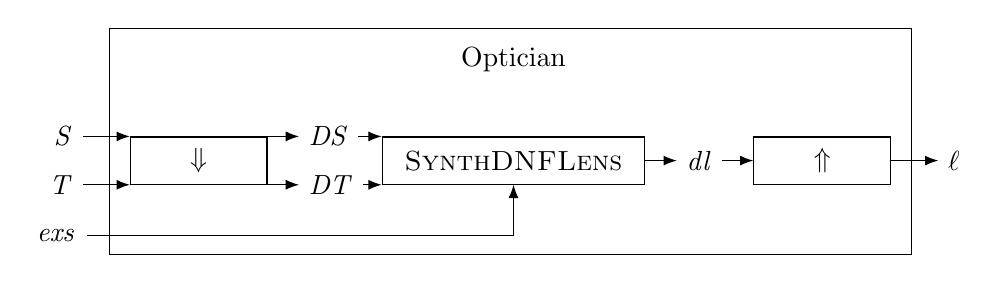
\begin{tikzpicture}[auto,node distance=1.5cm]
    \node[text width=1.5cm,minimum height=.6cm,align=center,draw,rectangle] (todnfregex) {\ToDNFRegex{}};
    
    \node[align=right, anchor=east] (regex1) [left = .6cm of todnfregex.north west]{\Regex{}};
    \node[align=right, anchor=east] (regex2) [left = .6cm of todnfregex.south west]{\RegexAlt{}};
    \node[align=right, anchor=east] (exs) [below = .2cm of regex2]{ \Examples{} };
    
    \node[align=center] (dnfregex1) [right = .4cm of todnfregex.north east]{\DNFRegex{}};
    \node[align=center] (dnfregex2) [right = .4cm of todnfregex.south east]{\DNFRegexAlt{}};

    \node[text width=3.1cm,minimum height=.6cm,align=center,draw,rectangle] [right = 1.45cm of todnfregex.east] (synthdnflens) {\SynthDNFLens{}};
    \node[align=center] [above = .7cm of synthdnflens] (optician) {\Optician{}};
    
    \node[align=center] [right = .4cm of synthdnflens] (dnflens) {\DNFLens{}};
    
    \node[text width=1.5cm,minimum height=.6cm,align=center,draw,rectangle] [right = .4cm of dnflens] (tolens) {\ToLens{}};
    
    \node[align=center] [right = .6cm of tolens] (lens) {\Lens{}};
    
    
    \path[->] (regex1.east) edge (todnfregex.north west);
    \path[->] (regex2.east) edge (todnfregex.south west);
    
    \path[->] (todnfregex.north east) edge (dnfregex1.west);
    \path[->] (todnfregex.south east) edge (dnfregex2.west);
    
    \path[->] (dnfregex1.east) edge (synthdnflens.north west);
    \path[->] (dnfregex2.east) edge (synthdnflens.south west);
    
    \path[->] (synthdnflens) edge (dnflens);
    
    \path[->] (dnflens) edge (tolens);
    
    \path[->] (tolens) edge (lens);
    \draw[->] ($(exs.east)+(-3pt,0)$) -| node(exsedge) {} (synthdnflens);
    \node[fit={($(todnfregex.west)+(-4pt,0)$) ($(tolens.east)+(4pt,0)$) (exsedge) (dnfregex1) (optician) (dnfregex2)},draw] (surrounding) {};
    % Now place a relation (ID=rel1)
    %\node[text width=2cm,align=center,draw, rectangle] (sketch-gen) [right = .75cm of spec] {\TypeProp{}};
    %\node (below-gen) [below=.5cm of sketch-gen] {};
    %\node[text width=2cm,align=center,draw, rectangle] (sketch-compl)
    %     [right = .25cm of sketch-gen] {\RigidSynth{}};
    %\node (below-compl) [below=.5cm of sketch-compl] {};
    %\node[align=center] (lens) [right = .75cm of sketch-compl] {Lens}; 
    %% Draw an edge between rel1 and node1; rel1 and node2
    %\path[->] (spec) edge node (start-alg) {} (sketch-gen);
    %\path[->] (sketch-gen) edge node(middle) {} (sketch-compl);
    %\path[->] (sketch-compl) edge node[near start](success) {\Success{}} (lens);
    %\draw[<-] (sketch-gen.south) -- +(0,-.5) -| node[above left](failure){\Failure{}} (sketch-compl.south);

    %\node (synth-name) [above=.5cm of middle] {\Optician{}};
    %
    %\node[fit=(sketch-gen) (sketch-compl) (start-alg) (synth-name) (failure)
    %(success) ,draw] (surrounding) {};

  \end{tikzpicture}
  \caption{Schematic Diagram for \Optician{}.  Regular expressions, \Regex{} and
    \RegexAlt{}, and examples, \Examples{}, are given as input.
    First, the function \ToDNFRegex{} converts \Regex{} and \RegexAlt{} into
    their respective DNF forms, \DNFRegex{} and \DNFRegexAlt{}.
    Next, \SynthDNFLens{} synthesizes a DNF lens, \DNFLens{}, from \Regex{},
    \RegexAlt{}, and \Examples{}.
    Finally, \ToLens{} converts \DNFLens{} into \Lens{}, a lens in Boomerang
    that is equivalent to \DNFLens{}.}
  \label{fig:schematic-diagram-synthesis}
\end{figure}

\Cref{fig:schematic-diagram-synthesis} shows a high-level,
schematic diagram for \Optician{}.
First, \Optician{} uses the function \ToDNFRegex{} to convert the input
regular expressions into DNF regular expressions.  Next,
\SynthDNFLens{} performs type-directed synthesis on these DNF regular
expressions and the input examples to synthesize a DNF lens.  Finally, this DNF lens is
converted back into a regular lens with the function \ToLens{}, and returned to the user.


\subsection{Quotient lens synthesis}

Quotient lenses are lenses in which the lens laws are
loosened so that they hold modulo an equivalence relation on the source and
target data respectively; as above, we are concerned with {\em bijective
quotient lenses} which are lenses for which Equation \ref{bijectivelenslaws}
holds modulo equivalence relations $\equiv_S$ and $\equiv_T$ defined on the source
and target data respectively:

\begin{equation}\label{quotientlenslaws}
\ell.\get \; (\ell.\lput \; t) \equiv_T t \text{, and } \ell.\lput \; (\ell.\get
\; s) \equiv_S s
\end{equation}

The inputs to the quotient lens synthesis problem, as in the bijective case,
include source and target regular expressions $S$ and $T$ and a set of example
instances.  The equivalence relations $\equiv_S$ and $\equiv_T$ are also given
as inputs to the synthesis algorithm.  Definition of such equivalences
are given via a new language of \textit{quotient regular expressions}
that we have defined.  Quotient regular expressions
describe both  $S$ (or $T$) and $\equiv_S$ (or $\equiv_T$)
simulataneously in one compact notation.

\subsection{Simple symmetric lens synthesis}
Although it is very useful to be able to synthesize bijective or
quotient lenses between data formats, such lenses do not fully solve the
problem. 
Bijective and quotient lenses require the two data formats to have
either precisely or morally the same information content. 
Many related data formats in practice have overlapping
information: some information may be present in one format but not the
other and vice versa.  

Symmetric lenses~\cite{HofmannPierceWagner10:POPL} address this
limitation.  General symmetric lenses introduce the notion of 
\textit{complement} that stores the information necessary to fully
reconstruct one format from the other.  Because such complements would
complicate the synthesis specificaiton problem, we instead define a
more restricted language of \textit{simple symmetric lenses}, which
are the largest class of symmetric lenses that do not rely on
persistent internal state to synchronise between two related data
formats, a property called \textit{forgetfulness}.  (Instead of a
complement, simple symmetric lenses rely on defaults to replace
missing information.)

A challenge in adopting the type-directed synthesis approach to simple
symmetric lenses is the number of such lenses.  Whereas the number of
bijective lenses between two formats is typically tiny, the
number of simple symmetric lenses is typically enormous. 
If a na\"ive  search algorithm just selects the first simple symmetric
lens it finds, the returned lens will generally not be the one the
user wanted. Symmetric synthesis requires a new principle for
identifying “more likely” lenses and a more sophisticated synthesis
algorithm that uses this principle to search the space more
intelligently.

For these, we turn to information theory. We consider ``likely'' lenses to
be ones that propagate ``a lot'' of information 
from the left data format to the right and vice versa. Conversely, ``unlikely''
lenses are ones that require a large amount of additional information to recover
one of the formats given the other. By default, our synthesis algorithm prefers
lenses that propagate more information.
This preference is formalized using \emph{stochastic regular expressions}
(SREs)~\cite{stoch-rnn,stoch-def}, which simultaneously define a set of
strings and a probability distribution over those strings.  Using this
probability distribution, we can calculate the likelihood of a given
lens.
We also allow users to override the default mechanism for
calculating the information content of a SRE by
asserting that certain strings are \emph{essential} or \emph{irrelevant},
forcing certain data to either be retained or discarded during the
transformations.



\begin{figure}
 \centering
  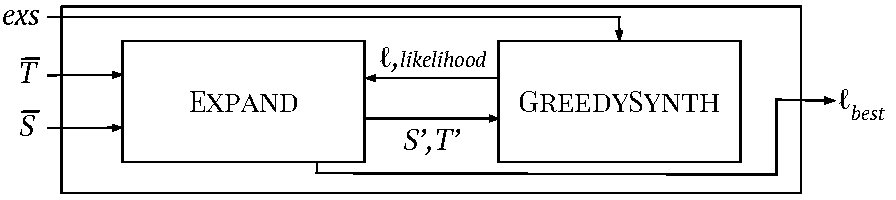
\includegraphics[width=.63\textwidth]{high-level-algorithm.pdf}
  \vspace{-2ex}
  \caption{Schematic diagram for the simple symmetric lens synthesis algorithm.
    The user provides regular expressions \BRegex and \BRegexAlt and a set of
    examples \Examples{} as input. \Expand first converts \BRegex and \BRegexAlt
    to stochastic regular expressions \Regex and \RegexAlt with default
    probabilities. It then finds pairs of stochastic regular expressions
    equivalent to \Regex and \RegexAlt and iteratively proposes them to
    \GreedySynth. \GreedySynth finds a lens typed between the supplied SREs.
    When the algorithm finds a likely lens, it returns it.}
  \label{fig:high-level-algorithm}
\end{figure}

With simple symmetric lenses and this SRE-based likelihood measure in hand, we
propose a new algorithm for synthesizing likely lenses. At its core, the
algorithm performs a type-directed search between descriptions of the data
formats, measuring success using the likelihood measure.

Interesting complications arise from the need to deal with regular-expression
equivalences. There are infinitely many regular expressions equivalent to a
given one, and the lens returned by a type-directed search will in general
depend on which of the possible representations are chosen for its source and
target formats. Moreover, certain lenses may not be well-typed unless the
format representations are replaced by equivalent ones:
in general, the synthesis algorithm has to search through
equivalent regular expression types to find the most likely lens. To tame
this complexity, we divide the synthesis algorithm into two communicating search
procedures (Figure~\ref{fig:high-level-algorithm}), following~\cite{optician}.
The first, \Expand, uses rewriting rules to propose new pairs of
stochastic regular expressions equivalent to the original pair. The second,
\GreedySynth, uses a greedy, type-directed
algorithm to find a simple symmetric lens between input SRE pairs, returning the lens and
its likelihood score to \Expand. The whole synthesis algorithm heuristically
terminates when a sufficiently likely lens is found.



\section{Results and Discussion}

% From bijective lens paper

% \newcommand{\SOptician}{Optician\textsubscript{S}}
% \newcommand{\SynthSymLens}{\PCF{SynthSymLens}\xspace}
% \newcommand{\RXSearchState}{\ensuremath{\mathit{pq}}}
% \newcommand{\ToStochastic}{\PCF{ToStochastic}\xspace}
% \newcommand{\LC}{\ensuremath{\mathit{lc}}}
% \newcommand{\Best}{\ensuremath{\mathit{best}}}
% \newcommand{\RXSearch}{\PCF{RXSearch}\xspace}
% \newcommand{\Continue}{\PCF{Continue}\xspace}
% \newcommand{\PQ}{\PCF{PQ}\xspace}
% \newcommand{\SynthDNFLens}{\PCF{SynthDNFLens}}
% \newcommand{\ToLens}{\ensuremath{\Uparrow}}
% \newcommand{\ToLensOf}[1]{\ensuremath{\ToLens{}\mkern-4mu #1}}
% \newcommand{\ToDNFRegexText}{\PCF{ToDNFRegex}}
% \newcommand{\Beautify}{\PCF{Beautify}}
% \newcommand{\RigidSynth}{\PCF{RigidSynth}}
% \newcommand{\GreedySynth}{\PCF{GreedySynth}\xspace}
% \newcommand{\RigidSynthInternal}{\PCF{RigidSynthInternal}}
% \newcommand{\RigidSynthSequence}{\PCF{RigidSynthSeq}}
% \newcommand{\RigidSynthAtom}{\PCF{RigidSynthAtom}}
% \newcommand{\GetDNFNormalizer}{\PCF{GetDNFNormalizer}}
% \newcommand{\CreatePQueue}{\PCF{CreatePQueue}}
% \newcommand{\GetTransitiveSet}{\PCF{GetTransitiveSet}}
% \newcommand{\GetCurrentSet}{\PCF{GetCurrentSet}}
% \newcommand{\Pop}{\PCF{Pop}}
% \newcommand{\ExpandOnce}{\PCF{ExpandOnce}}
% \newcommand{\ExpandRequired}{\PCF{ExpandRequired}}
% \newcommand{\FixProblemElts}{\PCF{FixProblemElts}}
% \newcommand{\Expand}{\PCF{Expand}\xspace}
% \newcommand{\ForceExpand}{\PCF{ForceExpand}}
% \newcommand{\Reveal}{\PCF{Reveal}}
% \newcommand{\Map}{\PCF{Map}}
% \newcommand{\EnqueueMany}{\PCF{EnqueueMany}}
% \newcommand{\ReturnVal}[1]{\ensuremath{\Return\,#1}}
% \newcommand{\CurrentSet}{\ensuremath{\mathit{CS}}}
% \newcommand{\TransitiveSet}{\ensuremath{\mathit{TS}}}

% \newcommand{\SSOpt}{\ensuremath{\mathbf{SS}}}
% \newcommand{\SSNCOpt}{\ensuremath{\mathbf{SSNC}}}
% \newcommand{\BSOpt}{\ensuremath{\mathbf{BS}}}
% \newcommand{\BSNCOpt}{\ensuremath{\mathbf{BSNC}}}
% \newcommand{\AnyOpt}{\ensuremath{\mathbf{Any}}}
% \newcommand{\FLOpt}{\ensuremath{\mathbf{FL}}}
% \newcommand{\CCOpt}{\ensuremath{\mathbf{DC}}}
% \newcommand{\NSOpt}{\textbf{NS}}
% \newcommand{\NROpt}{\textbf{NR}}

We implemented our synthesis algorithms in the OCaml programming language
and integrated them into Boomerang system, where they are available as open
source code~\cite{GitHub}\bcp{Two more pointers needed}.  Users of Boomerang
can write lenses by hand, specify them as synthesis tasks, or do a
combination of both.

We analyzed our algorithms theoretically, proving various soundness and
completeness results.  We also analyzed these algorithms empirically,
studying their impact on a range of real and synthetic benchmarks.  Our
results have been published in a series of conference papers and technical
reports~\cite{bijective-synthesis,quotient-synthesis,symmetric-synthesis}.
In the rest of this section, we summarize key results.

\subsection{Bijective Synthesis Algorithms}

We first show the effectiveness of the pure bijective synthesis
algorithm by evaluating its performance on a set of 39
benchmark programs.  
%
All evaluations were performed on a 2.5 GHz Intel Core i7 processor with 16 GB
of 1600 MHz DDR3 running macOS Sierra.

\paragraph*{Benchmark Suite Construction}
We constructed our benchmarks primarily by adapting examples from
Augeas~\cite{augeas} and 
Flash Fill~\cite{gulwani-popl-2014}.
%
Augeas is a configuration editing system for Linux that uses lens
combinators similar to those in Boomerang.  
% , with some small
% differences. However, it transforms 
% strings on the left to structured trees on the right rather than
% transforming strings to strings.
% We adapted these Augeas lenses to our setting by converting the
% right-hand sides to strings that correspond to serialized versions
% of the tree formats
We derived 29 of the benchmark tests by
adapting the first 27 lenses from the Augeas library in alphabetical order,
as well as the lenses 
\CF{aug/xml-firstlevel} and \CF{aug/xml} that were referenced
by the `A' lenses.
Furthermore, the 12 last synthesis problems derived
from Augeas were tested after our synthesizer was was
finalized, demonstrating that the optimizations were not
over-tuned to perform well on the testing data.
%
Flash Fill is a system that allows users to specify common string
transformations by example~\cite{gulwani-popl-2014}.  
We derived three benchmarks from the first few examples in this
paper and one from the running example on
extracting phone numbers.

Both Augeas and Flash Fill permit non-bijective transformations.
To test our system on these benchmarks, we had to convert them into
bijective transformations (by hand).  Specifically, in many of the
benchmarks, we normalized
the whitespace in the documents so the amount of whitespace was equal
in the source and target.  In a few of the benchmarks, either the
source or the target was missing information present in the other
format.  We modified those benchmarks by adding the missing
information back into the file. 

Finally, we added a few custom examples designed to highlight known
weaknesses of our algorithm
%(\CF{cap-prob} and \CF{2-cap-prob}) 
and to test situations for which we thought the tool would be
particularly useful.
% (\CF{workitem-probs}, \CF{date-probs}, \CF{bib-prob},
% and \CF{addr-probs}).
These examples convert between work item formats, date
formats, bibliography formats, and address formats, respectively.

\begin{figure}
  \centering
  \begin{subfigure}[b]{.49\textwidth}
    \centering
    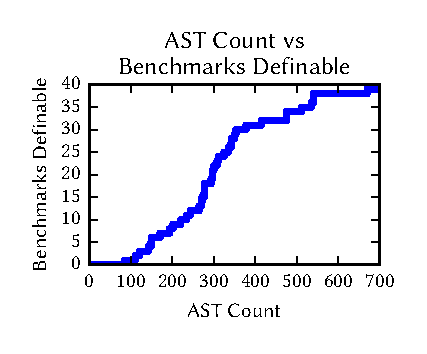
\includegraphics{figs/specsizes}
    \caption{}
    \label{subfig:lenssize}
  \end{subfigure}
  \begin{subfigure}[b]{.49\textwidth}
    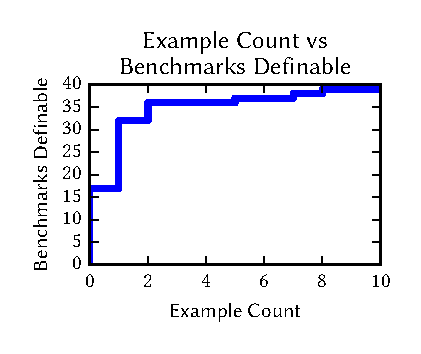
\includegraphics{figs/examplesused}
    \caption{}
    \label{subfig:examplesused}
  \end{subfigure}
  \caption{Sizes of Specifications.
    In (a), we show how many benchmarks are defined in our suite using a
    given number of AST nodes or fewer.
    In (b), we show how many benchmarks are defined in our suite using a
    given number of examples or fewer.}
  \label{fig:definition-sizes}
\end{figure}

Figure~\ref{fig:definition-sizes} shows the complexity of our type-based
specifications as well as our example counts.
An average benchmark has a type-based specification that can be represented using
310 AST node, and requires 1.1 input/output examples.
Our benchmarks vary from simple problems, like changing the
representation of dates
(with a specification size of 85, and a generated lens size of 79), to 
complex tasks, like transforming configuration files for server monitoring
software into dictionary form (with a specification size of 670 and
a generated lens size of 651).  On average, the size of the generated lens is
89\% the size of its type specifications.


\paragraph*{Importance of Examples}

\begin{figure}
  \centering
  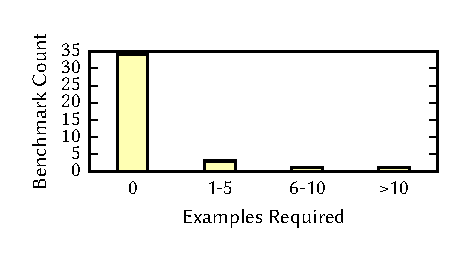
\includegraphics{figs/examples.eps}
  \caption{Average number of random examples required to synthesize benchmark
    programs.  {\bf Experimental Average} is the average number of randomly
    generated examples needed to correctly synthesize the lens.  {\bf
      Determinize Permutations} is the theoretical number of examples required
    to determinize the choice all the permutations in \RigidSynth{}.
    In practice, far fewer examples are
    needed to synthesize the correct lens than would be predicted by the number
    required to determinize permutations.}
  \label{fig:exs-reqd}
\end{figure}

To evaluate how many user-supplied examples the algorithm requires in
practice, we \textit{randomly} generated appropriate source/target
pairs, mimicking what a na\"{i}ve user might do.  We did not write the
examples by hand out of concern that our knowledge of the synthesis
algorithm might bias the selection. Figure~\ref{fig:exs-reqd} shows
the number of randomly generated examples it takes to synthesize the
correct lens averaged over ten runs.  The synthesis algorithm almost never needs
any examples: only 5 benchmarks need a nonzero number of examples to
synthesize the correct lens and only one, \CF{cust/workitem-probs} required over
10 randomly generated examples.
A clever user may be able to reduce the
number of examples further by selecting examples carefully; we
synthesized \CF{cust/workitem-probs} with only 8 examples.

These numbers are low because there are relatively few well-typed
bijective lenses between any two source and target regular expressions. 
As one would expect, the benchmarks where there are multiple ways to
map source data to the target (and vice versa) require the most examples.
For example, the benchmark \CF{cust/workitem-probs} requires a large number of
examples because it
must differentiate between data in different text fields in both the
source and target and map between them appropriately.  As these text fields are
heavily permuted
(the legacy format ordered fields by a numeric ID, where
the modern format ordered fields alphabetically) and fields can be
omitted, a number of examples are needed to correctly identify the mapping
between fields.

The average number of examples to
infer the correct lens does not tell the whole story.  The system will
stop as soon as it finds a well typed lens that satisfies the supplied examples.
This inferred lens may or may not 
correctly handle unseen examples that correspond to
unexercised portions of the source and target regular expressions.
Figure~\ref{fig:exs-reqd} lists
the number of examples that are required to determinize the generation of
permutations in \RigidSynth{}.
Intuitively, this number represents the maximum number of
examples that a user must supply to guide the synthesis engine if it
always guesses the wrong permutation when multiple permutations can be used to
satisfy the specification. 

The average number of examples is so much lower than the maximum
number of required examples because of correspondences in how we wrote
the regular expressions for the source and target data formats. 
Specifically, when we had corresponding disjunctions in both the
source and the target, we ordered them the same way.  The algorithm
uses the supplied ordering to guide its search, and so the system
requires fewer examples.   We did not write the examples in this style
to facilitate synthesis, but rather because maintaining similar
subparts in similar orderings makes the types much easier to 
read. We expect that most users would do the same.

\paragraph*{Comparison Against Other Tools}
%
We are the first tool to synthesize bidirectional transformations between data
formats, so there is no tool to which we can make an apple-to-apples comparison.
Instead, we compare against tools for generating unidirectional
transformations instead. 
Figure~\ref{fig:synthesis-times} includes a comparison against two other
well-known tools that synthesize
text transformation and extraction functions from examples -- Flash Fill and FlashExtract.  For this
evaluation, we used the version of these tools distributed through the
PROSE project~\cite{prose}.

\begin{figure}
  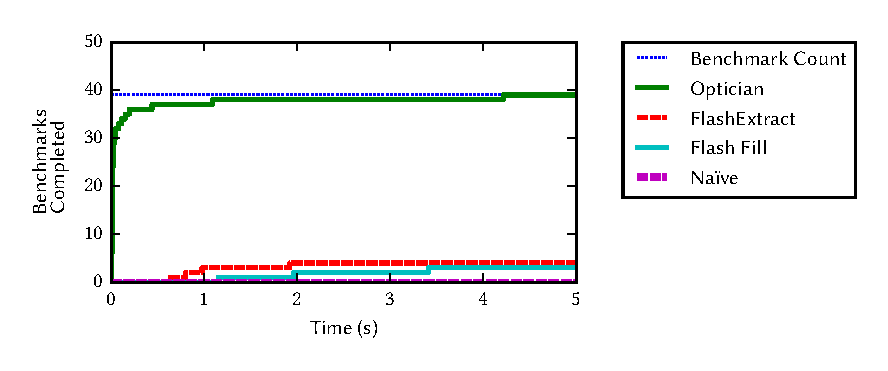
\includegraphics{figs/times}
  \caption{
    Number of benchmarks that can be solved by a given algorithm in a given
    amount of time.
    \Optician{} is our bijective synthesis algorithm including a set
    of optimizations we have implemented.
    \FlashExtractMode{} is the existing FlashExtract system.  \FlashFillMode{} is
    the existing Flash Fill system.  \NaiveMode{} is na\"{i}ve type-directed 
    synthesis on the bijective lens combinators.  Our synthesis algorithm performs
    better than the na\"{i}ve approach and other string transformation systems,
    and our optimizations speed up the algorithm enough that all tasks become
    solvable.
  }
  \label{fig:synthesis-times}
\end{figure}

To generate specifications for Flash Fill, we generated input/output
specifications by generating random elements of the source language, and
running the lens on those elements to generate elements of the target language.
These were then fed to Flash Fill.

To generate specifications for FlashExtract, we extracted portions of strings
mapped in the generated lens either through an identity
transformation or through a previously synthesized lens, whereas strings that were
mapped through use of \ConstLens{} were considered boilerplate and so not
extracted.

As these tools were designed for a broader audience, they put less of a burden
on the user.  These tools only use input/output examples (for Flash
Fill), or marked text regions (for FlashExtract), as opposed
to \Optician{}'s use of regular expressions to constrain the format of
the input and output.  By using regular expressions,
\Optician{} is able to synthesize significantly more programs
than either existing tool.

Flash Fill and FlashExtract have two tasks: to determine how
the data is transformed, they must also infer the structure of the data, a
difficult job for complex formats.
In particular, neither Flash Fill nor FlashExtract was able to synthesize
transformations or extractions present under two iterations, a type of format
that is notoriously hard to infer.
These types of dual iterations are pervasive in Linux configuration
files, making Flash Fill and FlashExtract ill suited for many of the synthesis
tasks present in our test suite.

Furthermore, as unidirectional transformations, Flash Fill and FlashExtract have
a more expressive calculus.  To guarantee bidirectionality, our syntax must be
highly restrictive, providing a smaller search space to traverse.

\subsection{Quotient Synthesis Algorithms}

% DPW:  From Quotient lenses paper

\newcommand{\wf}[1]{\ensuremath{#1\;\mathsf{wf}}}

% FOR Regular Expression names
\newcommand{\re}[1]{\ensuremath{\mathtt{#1}}}
\newcommand{\codefont}[1]{\ensuremath{\mathsf{#1}}}
\newcommand{\kw}[1]{\textcolor{dkblue}{\ensuremath{\mathsf{#1}}}}
\newcommand{\collapse}[2]{\ensuremath{\kw{collapse} \; #1 \mapsto #2}}
\newcommand{\squash}[3]{\ensuremath{\kw{squash} \; #1 \rightarrow #2\; \kw{using} \; #3}}
\newcommand{\perm}[2]{\ensuremath{\kw{perm}(#1)\; \kw{with}\; #2}}
\newcommand{\normalize}[3]{\ensuremath{\kw{normalize}(#1, #2, #3)}}
\newcommand{\eqrel}[1]{\ensuremath{\equiv_{#1}}}

\newcommand{\canonize}{\ensuremath{\kw{canonize}}}

\newcommand{\Name}{Optometrist\xspace}

\newcommand{\QRESize}{\textbf{QS}}
\newcommand{\canonizeAndSpecSize}{\textbf{BS}}
\newcommand{\LensAndSpecSize}{\textbf{NS}}

%\newcommand{\QOpt}{Optician_Q}
\newcommand{\QOpt}{QRE-enhanced Optician}
\newcommand{\OpticianRuntime}{\textbf{Optician}}
\newcommand{\QREOptician}{\textbf{Optician\textsubscript{Q}}}
\newcommand{\SystemOnOptician}{\textbf{QO}}
\newcommand{\SystemOnBenchmarks}{\textbf{QQ}}
\newcommand{\cd}[1]{\lstinline[backgroundcolor=\color{white}]$#1$}

We have extended the bijective synthesis tool to synthesize quotient lenses. We will use 
``\QOpt'' to denote our extended version of Optician, and just plain ``Optician'' to denote
the pre-quotient version of Optician. The synthesis algorithm produces Boomerang lens
values, so Boomerang gives synthesized lenses the same first-class status as hand-written ones. 
%
All evaluations were performed on a 2.5 GHz Intel Core i7 processor with 16 GB
of 1600 MHz DDR3 running macOS High Sierra.


\paragraph*{Benchmark Suite Construction}

We analyzed the same 39 lens synthesis tasks from the original
Optician system.
We also experimented using our tool to synthesize quotient lenses
between XML, RDF and and JSON formats using data from the data.gov
database; the data consisted of census statistics, demographic
statistics, wage comparosion data, and crime index data).
Recall that to use bijective synthesis,  we had to modify 10 of 39
benchmarks make them bijective (for instance, by normalizing whitespace)
Because quotient lenses are more expressive, we were able avoid such
modifications. This
experience alone points to the benefits that quotient lens synthesis
brings to the table. 

\paragraph*{Evaluating programmer effort}

\begin{figure}[t]
\centering
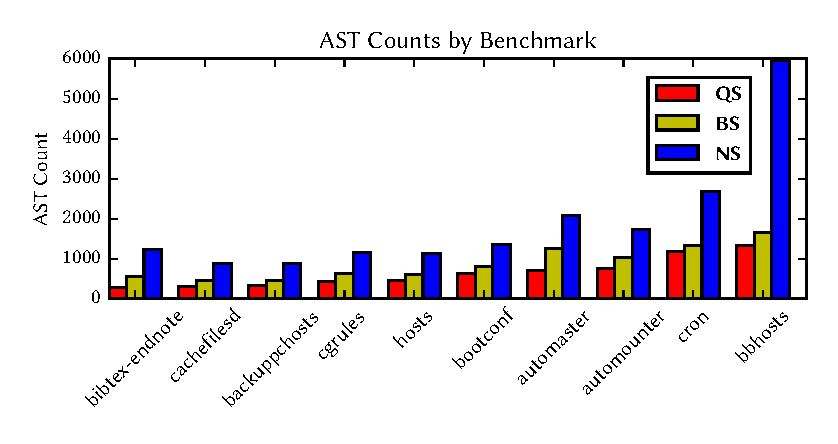
\includegraphics{qfigs/asts.eps}
\caption{AST node measurements for each of the three approaches
on each of the 10 non-bijective benchmark problems.
Benchmarks are sorted in order of increasing complexity as measured by
the number of AST nodes in the source and target format descriptions. 
QRE Synthesis requires far fewer AST nodes than the other
two approaches.}
%%\caption{Count of benchmark programs definable using a given AST count. We find
%%that it takes far fewer AST nodes to define benchmark lenses using QRE
%%synthesis than with Optician without QRE synthesis or without synthesis.}
\label{fig:asts}
\end{figure}

To evaluate the impact of QRE lens synthsis on programmer effort,
we focus our attention on the 10 problems in the benchmark suite that
are not bijective and hence require non-trivial canonizers. 
(Optician already handles the other problems with minimal programmer
effort.)

We are interested in comparing three different approaches, which vary
in the amount of synthesis used. 
In the first approach, which we call \QRESize{}, the programmer uses
quotient lens synthesis.  She must write QRE specifications of the source and
target formats and she may give examples.
In the second approach, which we call \canonizeAndSpecSize{} for
Bijective Synthesis, the
programmer uses bijective lens synthesis \`a la Optician.
She must write canonizers by hand, along with 
regular expressions to describe the external
representations of the source and target formats. (The internal
formats can be inferred from the canonizers.) She may also
provide examples to help in the synthesis of the bijective lens.
In the third approach, which we call \LensAndSpecSize{} for No Synthesis, the
programmer writes the lens between the source and target formats
entirely by hand, including the descriptions of the source and target
formats.

For each problem in the benchmark suite, we calculate the following
measures as proxies for the level of programmer effort when using each
the three approaches:

%
\begin{itemize}
  \item[\QRESize{}:] 
  The number of AST nodes in the QRE specifications for the source and
  target formats, including examples. 
  \item[\canonizeAndSpecSize{}:] 
  The sum of (1) the number of AST nodes in $W(q)$ for each QRE $q$ in the source and target
  formats, (2) the number of AST nodes in $\canonize(q)$ for each QRE $q$ with a
  non-trivial canonizer, and (3) the number of AST nodes in the
  examples.  We use (1) to estimate the burden of describing
  the external source and target formats and (2) to estimate the
  burden of writing the requisite canonizers
  by hand.  We count the nodes in the examples because they would be
  fed to the bijective synthesizer.  
  These counts are an approximation, as both $W(q)$ and $\canonize(q)$ are
  automatically generated from the corresponding QRE $q$, and it is
  possible that a human-written version might be smaller.
  \item[\LensAndSpecSize{}:] The sum of (1) the number of AST nodes in
  $W(q)$ for each QRE $q$ in the source and target formats and (2) the
  number of AST nodes in the synthesized QRE lens.  We use (1) to
  estimate the burdern of describing the source and target formats
  and (2) to estimate the burdern of writing the appropriate lens by
  hand. These counts are also approximations, as
  $W(q)$ and the synthesized lens may be larger than one written by hand.
\end{itemize}

Figure~\ref{fig:asts} shows each of these measures for the 10
non-bijective problems in the benchmark suite.  On
average (using a geometric mean), \canonizeAndSpecSize{} used~38.5\% more AST nodes
than \QRESize{}, requiring an average of~214 more AST nodes. On 
average, \LensAndSpecSize{} used~180\% more AST nodes than \QRESize{}, requiring an
average of~998 more AST nodes. These figures suggest that introducing QREs saves
programmers significant effort compared to both Optician and basic
Boomerang.

\paragraph*{Quotient Lens Performance}

\begin{figure}[t]
\centering
\begin{subfigure}[b]{.49\textwidth}
\centering
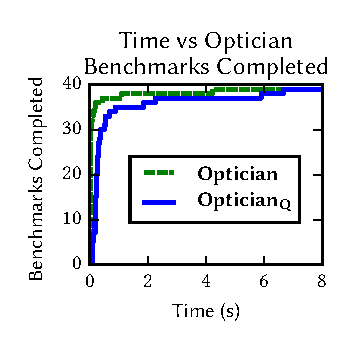
\includegraphics{qfigs/times_opt}
\caption{}
\label{subfig:lenssize}
\end{subfigure}
\begin{subfigure}[b]{.49\textwidth}
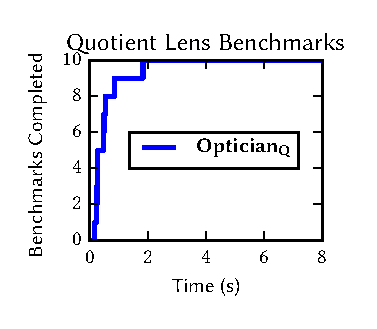
\includegraphics{qfigs/times_new.eps}
\caption{}
\label{subfig:examplesused}
\end{subfigure}
\caption{Runtime measurements. In (a), we run Optician and \QOpt{}
  on the Optician benchmarks.  We find that there is only a negligible
  performance overhead incurred by using QREs. 
  In (b), we run \QOpt{} on the 10 Optician benchmarks
  previously edited to make them bijective, after removing those edits
  and then extending the synthesis specification to include QREs.
  (In other words, we restored them to their original state, added QREs,
  and then ran \QOpt{}). 
  We find that \QOpt{} is able to
  synthesize all quotient lenses in under 10 seconds, and typically finishes in
  under 5 seconds.}
\label{fig:times}
\end{figure}

To assess the performance of quotient synthesis, we are interested in two different
questions. First, how does the performance of \QOpt{} compare to the performance
of Optician on benchmarks that do not require quotients? The answer to this question
tells us how much overhead we have introduced by adopting the more general
mechanism. Figure~\ref{fig:times}(a) shows that \QOpt{} was able to synthesize
all of the Optician benchmarks at a speed competitive with the old version.
There is a small amount of additional overhead introduced by QREs in calculating
equivalences, resulting in a slight decrease in performance.

Second, how much time does it take for \QOpt{} to synthesize a quotient
lens when running on a non-bijective benchmark problem?  
Figure~\ref{fig:times}(b) shows the amount of time required to infer a
lens for each of the 10 benchmark programs with nontrivial quotients.  
We find that \QOpt{} is able to synthesize all quotient lenses in
under 10~seconds, and typically finishes in under 5~seconds.

\subsection{Simple Symmetric Synthesis Algorithms}
We implemented simple symmetric lenses as an extension to
Boomerang~\cite{boomerang}.  
We also integrated our synthesis engine into Boomerang, allowing users
to write synthesis tasks 
alongside lens combinators, incorporate synthesis results into manually-written
lenses, and reference previously defined lenses during synthesis. All experiments
were performed on a 2.5 GHz Intel Core i7 processor with 16 GB of 1600 MHz DDR3
running macOS Mojave.

\paragraph*{Benchmark Suite Construction}
Our benchmarks are drawn from three different sources.
\begin{enumerate}
\item We adapted 8 data cleaning benchmarks from Flash Fill~\cite{flashfill}. Flash Fill data
  cleaning tasks are either derived from online help forums or taken from the
  Excel product team. Note that our tool produces bidirectional transformations
  rather than one-way transformers like Flash Fill. We ensure one direction of
  our bidirectional transformers performs the same unidirectional transformation
  as Flash Fill---the other direction is determined from the round-tripping
  laws. None of these benchmarks were bijective.
\item We adapted 29 benchmarks from Augeas~\cite{augeas}. Augeas is a utility
  that bidirectionally converts between Linux configuration files and an
  in-memory dictionaries. In our benchmarks, we synthesize lenses between Linux
  configuration files and serialized versions of Augeas dictionaries. Because
  these benchmarks merely transformed the information into a structured form,
  synthesized lenses were all bijective.
\item We created 11 additional benchmarks 
  derived from real-world examples and/or the bidirectional programming
  literature. These tasks range from synchronizing REST and JSON web resource
  descriptions to synchronizing BibTeX and EndNote citation descriptions. Five
  of these benchmarks were not bijective lenses.
\end{enumerate}

\paragraph*{Synthesizing Correct Simple Symmetric Lenses}

To determine whether the system can synthesize desired lenses, we ran
it interactively on all 48 benchmark tasks, working with the system to
create sufficient examples and provide useful relevance annotations
(\IE, \emph{essential} and \emph{irrelevant} markings, written as
\SRequire and \Skip, respectively).
In all cases, the desired lens was obtained.
%
The majority of the tasks required only a single example and none required
more than three examples to synthesize the desired lens.
%
Providing relevance annotations 
was needed in only 8 of the 48 tasks. In
practice, we found that adding such annotations was quite easy: if manual inspection
of the lens showed there were too few \IdentityLens{}s, and too many
\Disconnect{}s\footnote{
A \Disconnect{} is a lens combinator that marks a place where
information appears in one format but not the 
other: there is a \emph{disconnect} between the two formats. 
}
  or merges, we would add \SRequire annotations. If synthesis took
too long, we would add \Skip annotations.
%
We verified that the default running mode of our synthesis tool
(\SSOpt{}) generated the 
correct lenses the way programmers often validate their programs: we
manually inspected the code and ran unit tests on the synthesized
code. To determine whether the synthesis procedure generated the
correct lens when running in modes other than \SSOpt{}, we compared
generated lens to the lens synthesized by \SSOpt{}.


\paragraph*{Effectiveness of Optimizations in Simple Symmetric Synthesis}

Having determined appropriate examples and annotations for the 48
benchmarks, we evaluate the performance of the system by measuring the running
time of our algorithm in two modes:
\vskip .5ex
\begin{tabulary}{\linewidth}{rL}
  \SSOpt{}: & Run the symmetric synthesis algorithm with all optimizations enabled.\\
  \SSNCOpt{}: & Run the symmetric synthesis algorithm with no compositional synthesis enabled.\\
\end{tabulary}\\
\noindent
Compositional synthesis allows users to break a benchmark into a
series of smaller synthesis tasks, whose solutions are utilized in more complex
synthesis procedures. Compositional synthesis (\SSOpt{} mode)
allows our system to scale to arbitrarily large and complex formats; measuring
it shows the responsiveness of the system when used as
intended. \SSNCOpt{} mode, which synthesizes a complete lens all at once,
provides a useful experimental stress test for the system.

\begin{figure}
  \centering
  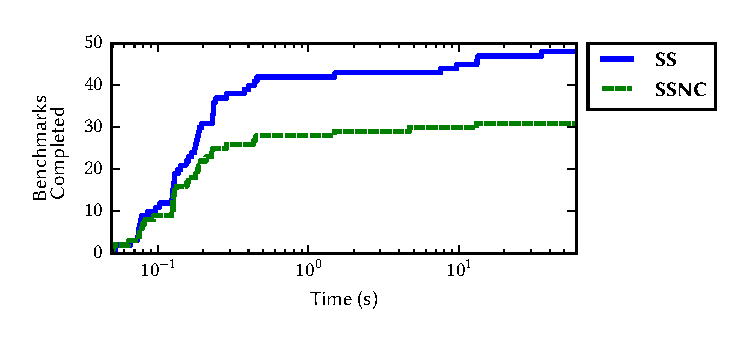
\includegraphics{times}
  \vspace{-2ex}
  \caption{Number of
    benchmarks that can be solved by a given algorithm in a 
    given amount of time. \SSOpt{} is the full symmetric synthesis algorithm.
    \SSNCOpt{} is the symmetric synthesis algorithm without using a library of
    existing lenses. The symmetric synthesis algorithm is able to complete all
    benchmarks in under 30 seconds elapsed total time. Without compositional
    synthesis it is able to complete 26. Each benchmark specification includes
    source and target (potentially annotated) regular expressions, and between
    one and three sufficient examples.}
  \label{fig:times}
\end{figure}

For each benchmark in the suite and each mode, we ran the system with a timeout
of 60 seconds, averaging the result over 5 runs. Figure~\ref{fig:times}
summarizes the results of these tests. We find that our algorithm is able to
synthesize all of the benchmarks in under 30 seconds. Without compositional
synthesis, the synthesis algorithm is able to solve 26 out of 48 problem instances.

% Section~\ref{subsec:optimizations} that users may tune the termination metric.
% Success on this set of benchmarks requires we tune that termination condition
% (e.g. for some benchmarks, allowing the system flexibility to spend more time
% considering more of the search space). In

\paragraph*{Slowdown Compared to Bijective Synthesis}

To compare to the existing bijective synthesis algorithm, we run our symmetric
synthesis algorithm on the original Optician benchmarks, comprised of
39 bijective synthesis tasks.\footnote{We had to slightly alter four of these
benchmarks, either by providing additional examples or by adding \SRequire annotations.
Without these alterations, symmetric synthesis yielded a lens that fit
the specification but that was undesired.}
To perform this comparison, we synthesized lenses in two modes:
\vskip 2ex
\begin{tabulary}{\linewidth}{rL}
  \BSOpt{}: & The existing bijective synthesis
              algorithm with all optimizations enabled.\\
  \SSOpt{}: & The symmetric synthesis algorithm with all optimizations enabled.\\
\end{tabulary}\\[2ex]
\noindent
For each benchmark, we ran it in both modes with a
timeout of 60 seconds and averaged the result over 5 runs.
Figure~\ref{fig:times_bijective} summarizes the results of these tests. On
average, \SSOpt{} took 1.3 times (0.5 seconds) longer to complete than
\BSOpt{}. The slowest completed benchmark for both synthesis algorithms is
\texttt{xml\_to\_augeas.boom}, a benchmark that converts arbitrary XML up to
depth 3 into a serialized version of the structured dictionary representation
used in Augeas. This benchmark takes 18.9 seconds for the symmetric synthesis
algorithm to complete, and 9.3 seconds the bijective synthesis algorithm to
complete. 

\begin{figure}[t]
  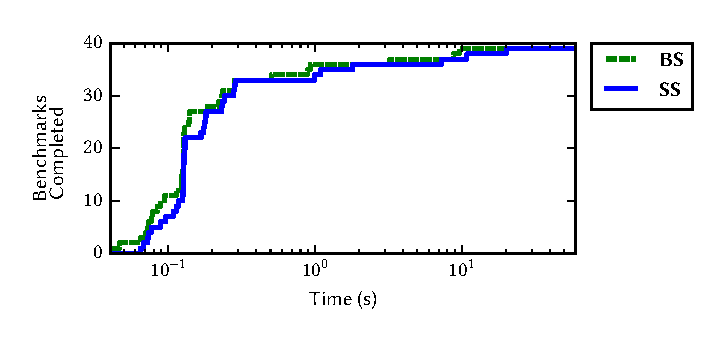
\includegraphics{times_bijective}
  \vspace{-2ex}
  \caption{Number of benchmarks that can be solved by a given algorithm in a
    given amount of time. \SSOpt{} is the full symmetric synthesis algorithm.
    \BSOpt{} is the full bijective lens synthesis algorithm.}
  \label{fig:times_bijective}
\end{figure}


\paragraph*{The Effects of Heuristics and Relevance Annotations}
We evaluate the usefulness of (1) our information-theoretic metric, (2) our
termination heuristic and (3) our
relevance annotations.  To this end, we run our program in several different modes:\\[2ex]
\begin{tabulary}{\linewidth}{rL}
  \AnyOpt{}: & Ignore the information-theoretic metric (\IE, all valid
               lenses have cost 0). \\ 
  \FLOpt{}: &  Return the first highest ranked lens \GreedySynth returns (\IE,
              ignore the termination heuristic). \\
  \CCOpt{}: & Replace our information-theoretic cost metric with one where
              the cost of the lens is the number of disconnects plus the number
              of merges.\\
  \NSOpt{}: & Ignore all \Skip annotations in the SRE specifications. \\
  \NROpt{}: & Ignore all \SRequire annotations in the SRE specifications. \\[2ex]
\end{tabulary}

\noindent
We experimented with the \CCOpt{} mode to determine whether the
complexity of the information-theoretic measure was really
needed. Related work on string transformations has often used simpler
measures such as ``avoid constants'' that align with, but are simpler
than our measures. The \CCOpt{} mode is an example of such a simple
measure---it operates by counting disconnects, which put a complete
stop to information transfer, and merges, which
eliminate the information in a union. 

\begin{figure}[t]
  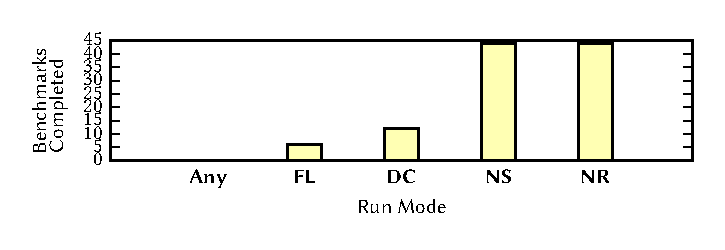
\includegraphics{metrics_importance}
  \vspace{-2ex}
  \caption{Number of benchmarks that synthesize the correct lens by a given
    algorithm. \AnyOpt{} provides no notion of cost, and merely returns the
    first lens it finds that satisfies the specification. \FLOpt{} provides a
    notion of cost to \GreedySynth, but once a satisfying lens is greedily
    found, that lens is returned. \CCOpt{} synthesizes lenses, where the cost of
    a lens is the number of disconnects plus the number of merges. \NSOpt{}
    ignores all \Skip annotations while running the algorithm. \NROpt{} ignores
    all \SRequire annotations while running the algorithm.}
  \label{fig:metric}
\end{figure}

Figure~\ref{fig:metric} summarizes the result of these experiments. The data
reveal that the information-theoretic metric is critical for finding the correct
lens: Only 10 of the benchmarks succeeded when running in \CCOpt{} mode. The
termination condition is also quite important. When running in \FLOpt{} mode,
the algorithm only discovers 5 lenses, which shows that the first class that
contains a satisfying lens is rarely the correct class. However, our algorithm
is not perfect and fails when either it is very difficult to find the desired
lens (necessitating \SRequire) or when a large amount of data is projected
(necessitating \Skip). Without any annotations, our algorithm finds the correct
lens for 40 of our 48 benchmarks; eight required relevance annotations to find
the correct lens.
% end evaluation

\section{Conclusions}

In this project, we designed, analyzed and implemented algorithms that
synthesize three classes of bidirectional transformations: (1) pure
bijective transformations, (2) bijections modulo equivalences classes
(quotient lenses) and (3) bijections modulo projections (simple symmetric
lenses).  Our synthesis algorithms take as inputs a format specification
(which includes specification of equivalence classes) and a collection of
examples.  As the class of transformations becomes richer, the number of
potential programs grows dramatically.  As a result, the corresponding
inference algorithm slows and its ability to guess the transformation
desired by the user decreases, leading to reduced accuracy.  We overcame
these challenges through new heuristics that use information theory to help
guide the search for program transformations.  In addition, to scale our
prototype to larger transformation tasks, we found it necessary to work
compositionally, by breaking down complex synthesis tasks into smaller, more
mangeable subtasks.

\bibliographystyle{apalike}
\bibliography{local.bib,bcp.bib}

\section{List of Symbols, Abbreviations, and Acronyms}
\begin{longtable}{p{1in}p{5in}}
  \ToDNFRegex{}         & An operation that converts regular   expressions into DNF form\\
  \ToLens{}             & An operation that converts a DNF lens to a  lens \\
  $\equiv_S$, $\equiv_T$ & Equivalence relations on data matching
                           regular expressions $S$ and $T$
                           respectively \\
  \AnyOpt{}             & Mode for simple symmetric synthesis that ignores the information-theoretic metric \\ 
  AST     & Abstract syntax tree\\  
  \BSOpt{}              & Bijective lens synthesis algorithm\\
  DARPA   & Defense Advanced Research Project Agency \\
  \CCOpt{}              & Mode for simple symmetric synthesis that
                          replace our information-theoretic cost metric with one where 
                          the cost of the lens is the number of disconnects plus the number
                          of merges.\\
  \DNFLens{}            & Lens in disjunctive normal form\\
  DNF                   & Disjunctive normal form\\
  \DNFRegex{}, \DNFRegexAlt{}  & Regular expression in disjunctive normal form\\
  \Examples{}           & Examples \\
  \Expand       & A component of the synthesis algorithm that proposes candidate
                  types equivalent to the input \\
  \FLOpt{}              & Mode for simple symmetric synthesis that
                          returns the first highest ranked lens found
                          by  \GreedySynth \\
  \footnotesize{\GreedySynth} & Synthesis procedure that searches greedily for candidate
                 solutions \\
  HR & Human Resources \\
  HTML & Hyptertext Markup Language \\
  JSON & JavaScript Object Notation---a standard file format used to
         encode data objects\\
  \Lens{}               & A lens \\
  $\mathcal{L}(\BRegex{})$  & The language of strings for the regular expression
                             \BRegex{} \\
  \NROpt{}              & Mode for simple symmetric synthesis that
                          ignores all \SRequire annotations in the SRE specifications. \\
  \NSOpt{}              & Mode for simple symmetric syntehsis that
                          ignores all \Skip annotations in the SRE specifications. \\ 
  \Optician{} & Our prototype implementation of the lens synthesis algorithms \\
  QRE                   & Quotient regular expression\\
  \textbf{QS}  & Number of nodes in the abstract syntax of QRE specifications \\
  RDF & Resource Description Framework---used to model web resources \\
  REST & Representational State Transfer\\
  SRE                   & Stochastic regular expression\\
  \BRegex and \BRegexAlt & Regular expressions provided by the user\\
  \Regex{}, \RegexAlt{} & Regular expressions\\
  $S \Leftrightarrow T$ & Type of a lens that maps between data
                          described by regular expressions $S$ and $T$\\
  \SSOpt{}              & Full symmetric synthesis algorithm\\
  \SSNCOpt{}            & Symmetric synthesis algorithm without using a library of
    existing lenses.\\
  {\footnotesize \SynthDNFLens{}} & A type-directed lens synthesis algorithm \\
  XML & Extensible Markup Language---used in web services \\
\end{longtable}

\end{document}

%%% Local Variables:
%%% mode: latex
%%% TeX-master: t
%%% End:
